\documentclass[11pt]{amsart}
% Shared preamble of main.tex and supplement.tex. Load after the document class.
\usepackage{amsmath,amssymb,amsthm,mathtools}
\allowdisplaybreaks[1]
\usepackage[margin=1.1in]{geometry}
\setlength{\emergencystretch}{3em}
\sloppy
\usepackage{booktabs,longtable}
\usepackage{xr-hyper}
\usepackage[hidelinks]{hyperref}
\usepackage{refcount}
\usepackage{enumitem}

% ---------------------------------------------------------------- theorem environments
\newtheorem{theorem}{Theorem}[section]
\newtheorem{proposition}[theorem]{Proposition}
\newtheorem{lemma}[theorem]{Lemma}
\newtheorem{corollary}[theorem]{Corollary}
% Lettered results A--G of the introduction.
\newtheorem{maintheorem}{Theorem}
\newtheorem{mainproposition}[maintheorem]{Proposition}
\newtheorem{maincorollary}[maintheorem]{Corollary}
\renewcommand{\themaintheorem}{\Alph{maintheorem}}
\theoremstyle{definition}
\newtheorem{definition}[theorem]{Definition}
\newtheorem{construction}[theorem]{Construction}
\theoremstyle{remark}
\newtheorem{remark}[theorem]{Remark}

% ---------------------------------------------------------------- notation
\newcommand{\R}{\mathbb{R}}
\newcommand{\C}{\mathbb{C}}
\newcommand{\Z}{\mathbb{Z}}
\newcommand{\Q}{\mathbb{Q}}
\newcommand{\N}{\mathbb{N}}
\newcommand{\CP}{\mathbb{CP}}
\newcommand{\eps}{\varepsilon}
\newcommand{\Rcal}{\mathcal{R}}
\newcommand{\Hb}{H_{\mathrm b}}            % base area profile
\newcommand{\Pb}{P_{\mathrm b}}            % unused area
\newcommand{\Bo}{B^{\circ}}                % open capacity ball
\newcommand{\EB}{\mathbb{B}}               % Euclidean ball (radius)
\newcommand{\Pack}{\mathrm{Pack}}          % packing specification
\newcommand{\Hfin}{H_{\mathrm{fin}}}
\newcommand{\defdesc}{\operatorname{the}}   % definite description (never \the, a TeX primitive)
\DeclareMathOperator{\vol}{vol}

% ---------------------------------------------------------------- Lean / blueprint annotations
% \lean{...} (optionally [full] or [needed]) and \leanmark{...} attach Lean declaration names to the
% statement they are in. They print nothing: the names and coverage classes are indexed in
% verification/PAPER-INDEX.md, and the formal counterparts of the main results are listed in the
% section on formal verification. A coverage class other than full or needed is an error.
\newcommand{\lean}[2][]{\if\relax\detokenize{#1}\relax\else
  \ifcsname leancoverage@#1\endcsname\else
    \PackageError{paper}{Unknown Lean coverage `#1'}{Use full or needed.}\fi\fi\ignorespaces}
\expandafter\def\csname leancoverage@full\endcsname{}
\expandafter\def\csname leancoverage@needed\endcsname{}
\newcommand{\leanmark}[1]{\ignorespaces}
\newcommand{\uses}[1]{}
\newcommand{\proves}[1]{}

% ---------------------------------------------------------------- cross-document references
% Numbers of the other document carry a prefix: S for the supplement, M for the main text.
% In the main text: \Sref{Lemma}{lem:shd-foo} -> "Lemma S6.3"; \Ssec{sec:shd} -> "\S S6".
% In the supplement: \Mref{Lemma}{lem:eff-gronwall} -> "Lemma M7.1"; the lettered results of
% the main text keep their letters: \Mref{Theorem}{thm:main} -> "Theorem C".
% The second argument is the label WITHOUT the S-/M- prefix.
\makeatletter
\DeclareRobustCommand{\Mprefix}[1]{\edef\@Mref{\getrefnumber{M-#1}}\expandafter\@Mprefix\@Mref\@nil}
\def\@Mprefix#1#2\@nil{\ifnum`#1<`A M\fi}
\makeatother
\newcommand{\Snum}[1]{\href[page=\getpagerefnumber{S-#1}]{supplement.pdf}{S\ref*{S-#1}}}
\newcommand{\Mnum}[1]{\href[page=\getpagerefnumber{M-#1}]{main.pdf}{\Mprefix{#1}\ref*{M-#1}}}
\newcommand{\Sref}[2]{#1~\Snum{#2}}
\newcommand{\Ssec}[1]{\S\Snum{#1}}
\newcommand{\Mref}[2]{#1~\Mnum{#2}}
\newcommand{\Msec}[1]{\S\Mnum{#1}}

\hypersetup{
  pdftitle={Explicit Hamiltonian full packings of the four-ball by equal balls},
  pdfauthor={Liang Song},
  pdfsubject={Explicit symplectic ball packings and Lean 4 formal verification},
  pdfkeywords={symplectic geometry, Hamiltonian dynamics, ball packing, Lean 4},
  pdflang={en-US}
}
\usepackage{tikz}
\usepackage{array}
\newcolumntype{L}[1]{>{\raggedright\arraybackslash}p{#1}}
\externaldocument[S-]{build/supplement}[supplement.pdf]
\renewcommand{\topfraction}{.9}\renewcommand{\bottomfraction}{.8}\renewcommand{\textfraction}{.07}\renewcommand{\floatpagefraction}{.75}

\title[Explicit Hamiltonian packings of the four-ball]{Explicit Hamiltonian full packings of the four-ball\\ by equal balls}
\author{Liang Song}
\email{sl12160010@gmail.com}
\thanks{Version 1.1; supersedes version 1.0.1 (29 October 2026,
DOI~\href{https://doi.org/10.5281/zenodo.23763498}{10.5281/zenodo.23763498}) of ``Explicit Hamiltonian ball packings in
every dimension''.}
\date{}

\begin{document}
\begin{abstract}
For every $k\ge10$ and $\eps\in(0,1)$ we construct an explicit smooth compactly supported Hamiltonian $H_{k,\eps}$ on
$\R\times\R^4$ whose time-one map carries the $k$ closed unit balls centred at $(3i-3,0,0,0)$ into the ball of radius
$R=(k/(1-\eps/4))^{1/4}$, filling the fraction $1-\eps/4$. Such packings were previously known to exist only through
Biran's theorem, whose proof does not produce the embeddings, and explicitly only for square $k$. This answers the
mathematical part of Epoch AI's construction problem. The two main ingredients are a linear comparison function for which the increasing
rearrangement of the profile defect is exactly linear, in place of a contraction fixed point, and a return from the
Fermat cubic disc-bundle model to the ball, in which a cube-root symmetry proves avoidance of the line at infinity.
The construction brings to dimension four the twisted disc-bundle mechanism that a 2026 preprint of OpenAI introduced in
dimensions $2n\ge6$, and uses neither $J$-holomorphic curves nor Seiberg--Witten theory. We also
prove robustness under perturbation with an explicit margin. The main theorems are verified in Lean~4. General
capacities, $k=9$, higher dimensions and an algorithm with finite output are treated in a companion paper.
\end{abstract}
\maketitle

\section{Introduction}\label{sec:intro}

\subsection{The result}\label{sec:intro-problem}

Points of $\R^{2n}=\C^n$ are $z=(z_1,\dots,z_n)$, $z_j=x_j+iy_j$, with symplectic form
$\omega_0=\sum_jdx_j\wedge dy_j$. The Hamiltonian vector field of a function $H(t,z)$ is defined by
$\iota_{X_H}\omega_0=dH$, i.e.\ $X_H=(\partial_{y}H,-\partial_{x}H)$, and $\phi^t_H$ denotes its flow from time $0$ to
time $t$. We write $B(c)=\{\pi|z|^2\le c\}$ for the closed ball of capacity $c$, $\Bo(c)$ for its interior, and
$B(s,c)=s+B(c)$. Thus $B(s,\pi)$ is the closed unit ball about $s$, and $\Bo(\pi R^2)$ is the open Euclidean ball of
radius $R$ about the origin.

\begin{maintheorem}[Equal balls in the four-ball]\label{thm:intro-4d}
\uses{def:ham-H-final, def:intro-spec, prop:cmp-linear, prop:ham-embeddings, prop:ham-end}
Let $k\ge10$ be an integer and $\eps\in(0,1)$. Put
\[
 R=\left(\frac{k}{1-\eps/4}\right)^{1/4},\qquad C=\pi R^2,\qquad s_i=(3i-3,0,0,0)\in\R^4\quad(1\le i\le k),
\]
and $H_{k,\eps}=H[2,k,C,(\pi,\dots,\pi),(s_1,\dots,s_k)]$ (Definition~\ref{def:ham-H-final}). Then $H_{k,\eps}$ is
$C^\infty$ on $\R\times\R^4$, vanishes for $t\notin(0,1)$ and outside $\R\times\mathcal S$ for an explicit compact set
$\mathcal S$, and satisfies $\Pack(2,k,C,(\pi,\dots,\pi),s)$ (Definition~\ref{def:intro-spec}): its flow is global, and
its time-one map sends each closed unit ball $B(s_i,\pi)$ into $\Bo(\pi R^2)$, with pairwise disjoint images. Moreover
$k/R^4=1-\eps/4>1-\eps$.
\leanmark{four\_dim\_theorem, main\_time\_support, main\_support\_radius, flow\_images\_disjoint}
\end{maintheorem}

\begin{proof}
The centres are at distance at least $3$, so the closed unit balls are disjoint. Since $R^4=k/(1-\eps/4)>k\ge10$, we
have $k\pi^2<\pi^2R^4=C^2$ and $3\pi<\pi R^2=C$, so $(2,k,C,(\pi,\dots,\pi))$ is admissible
(Definition~\ref{def:intro-admissible}). The normalised capacity $\rho=\pi/C=R^{-2}$ satisfies
$\rho\sqrt k=\sqrt{1-\eps/4}>\sqrt3/2>\frac34$, so the data lie in the linear branch, which uses the linear
comparison datum of Proposition~\ref{prop:cmp-linear}. The proof is completed in \S\ref{sec:ham-proof-main}.
\end{proof}

The Hamiltonian is defined by the same formulas for all $(k,\eps)$. It is built from closed formulas, integrals,
time-one maps of explicit vector fields, inverses of explicit injective maps and extrema over explicit compact sets,
the operations of level L1 in Definition~\ref{def:intro-levels} (Table~\ref{tab:ham-explicit}).

The companion paper~\cite{SongHD} defines $H[n,k,C,c,s]$ for all admissible data and proves the packing for unequal
capacities in dimension four ($\sum_ic_i^2<C^2$, $3c_i<C$), for $k=9$ equal balls and in every dimension $2n\ge6$; it
also gives a uniform algorithm whose output is a rational polynomial times a fixed cutoff. The two papers supersede
the single paper~\cite{SongAll}.

\emph{The Epoch problem.} Epoch AI \cite{Epoch} asked for an algorithm that, on input $k\ge10$ and $\eps\in(0,1)$,
outputs an explicit smooth Hamiltonian on $\R^4$ whose time-one map sends the closed unit balls centred at
$(3i-3,0,0,0)$ into a closed ball $B^4(R)$ about the origin with $k/R^4>1-\eps$. Theorem~\ref{thm:intro-4d} and
Proposition~\ref{thm:intro-stability} answer the mathematical part of this construction problem; the algorithm with
finite output is in~\cite{SongHD}. Epoch also asks for a PyTorch implementation that a numerical verifier integrates within fixed time limits; the
construction here is designed for proof, not for fast integration. Two accompanying programs in the repository address
numerical evaluation: one in Epoch's Hamiltonian interface, built from the elementary constructions of the third paper
of the release (``Elementary packings of the four-ball and their limits'') over a covered range of $(k,\eps)$, and one
evaluating closed-form $C^4$ packing embeddings directly for every $k\ge10$ and $\eps\in(0,1)$ (proved in the fourth
paper of the release, ``Closed-form symplectic packings of the four-ball by equal balls'').

\subsection{What was known}\label{sec:intro-prior}

Balls of capacities $c_1,\dots,c_k$ embed disjointly in $\Bo(C)\subset\R^4$ only if $\sum_ic_i^2<C^2$ and, by Gromov's
two-ball theorem \cite{Gromov1985}, $c_i+c_j<C$. McDuff and Polterovich \cite{McDuffPolterovich1994} related such
packings to blow-ups of $\CP^2$ and found the maximal densities for at most nine equal balls; Biran
\cite{Biran1997} proved that $k$ balls of capacity $c$ embed in $\Bo(C)$ whenever $k\ge9$ and $kc^2<C^2$; and the work
of McDuff, Li--Liu and Li--Li \cite{McDuff1991,McDuff1998,LiLiu2001,LiLi2002} reduces every four-dimensional ball
packing problem to inequalities indexed by exceptional classes. Packing stability was extended by Biran \cite{Biran1999}, Buse, Hind and Opshtein
\cite{BuseHind2011,BuseHind2013,BuseHindOpshtein2016} and Edtmair \cite{Edtmair2025}, and fails for some open domains
\cite{CristofaroGardinerHind2023}. These proofs use $J$-holomorphic curves and, through Taubes' theorem and inflation,
Seiberg--Witten theory; they show that embeddings exist but do not produce a Hamiltonian moving given balls. Explicit
packings were known in special cases, and explicit full packings by $k\ge10$ equal balls only for square $k$: Traynor's full packings by $d^2$ equal balls \cite{Traynor1995}, folding,
wrapping and the cases $k\le9$ \cite{SchlenkHand,SchlenkBook,Schlenk2018}, tunnelling \cite{Wieck2009}, singular
curves and polarisations \cite{Opshtein2011,Opshtein2013}, and almost toric methods
\cite{Symington2003,CasalsVianna2020}. The OpenAI preprint \cite{OpenAI2026} proved the packing criterion conjectured by
Siegel and Yao \cite{SiegelYao2025} in dimensions $2n\ge6$; in dimension four the two inequalities are not a criterion. We use its twisted disc-bundle mechanism (whose comparison and surface lemmas allow fibres $\C^m$, $m\ge1$) and the
deformation-to-the-normal-cone scheme of its return. Dimension four needs a different model and new arguments: the
Fermat cubic disc bundle, the linear comparison identity, which replaces the fixed point by a closed formula, and the
symmetry argument that brings the model back to the ball.

The proof here uses explicit maps, forms and flows only, and none of the existence results above. It gives explicit
full packings of $B^4$, i.e.\ packings of every density below $1$, by $k\ge10$ equal balls without $J$-holomorphic curves or Seiberg--Witten theory. The
companion paper~\cite{SongHD} adds the scalar comparison datum, which covers $k=9$ and unequal capacities, and so
proves in the same way Biran's theorem \cite{Biran1997} that $B^4$ admits full packings by $k$ equal balls for every
$k\ge9$; the earlier proofs \cite{Biran1997,Biran1999,BuseHind2013,BuseHindOpshtein2016} use these tools, directly or
through the results they cite.

\subsection{The key ideas}\label{sec:intro-mechanism}

The model is Biran's decomposition of $\CP^2$ along a smooth cubic $E$ \cite{Biran2001}: the complement of an
isotropic skeleton is the degree-$9$ disc bundle over $E$ with fibres of capacity $\frac13$, and its base area at
fibre moment $p$ is $A(p)=3(1-3p)$. Balls are placed fibrewise; for $k\ge10$ balls of capacity close to $1/\sqrt k$ the
volume budget holds but the slice profile $\sum_i(a_i-p)_+$ exceeds $A(p)$ near $p=0$ (Figure~\ref{fig:intro-profile}).
Following \cite{OpenAI2026}, the bundle is twisted across an annulus in the base by an area-preserving map $q$ of the
fibre disc. Paired with a function $K$ of the moment, the twist moves base area between moment levels, and the balls fit
if, for $P=A-\sum_i(a_i-p)_+$ and some gap $\gamma>0$,
\[
 (K-P)\bigl(p(q(w))\bigr)\le K\bigl(p(w)\bigr)-\gamma\qquad\text{for every fibre point }w
\]
(Section~\ref{sec:mech}). In \cite{OpenAI2026} the function $K$ is the fixed point of a contraction built from
increasing rearrangements, and the planar maps realising the rearrangements and the relative Moser isotopies are
obtained from existence statements. Two ideas make the four-dimensional construction
explicit.

\emph{The linear comparison identity} (\S\ref{sec:cmp-linear}). For $k\ge10$ equal balls of capacity $a=t_0/\sqrt k$,
with the bundle cut at fibre moment $h=t_0/3$, the function $K-P$ with $K$ linear of slope $3\sqrt k-9$ is, up to the constant $-g$, a
multiple of a tent $\Lambda$ with $\Lambda(0)=\Lambda(h)=h$. Because the tent reaches the same height at both ends, each
sublevel interval $\{\Lambda\le b\}$ has length exactly $b$, so the increasing rearrangement of $\Lambda$ is the identity
and the comparison inequality reduces to the constant gap $g=3(1-t_0)$. One explicit planar map realises the
rearrangement at a cost of at most $g/32$. No fixed point is needed.

\emph{The return to the ball} (\S\ref{sec:mdl-return}). The disc bundle is written by theta functions on the cover
$\R^2\times\C$ of the Fermat torus and carried into $\CP^2$ by explicit injection, transport and Moser flows. The ball is
$\CP^2$ minus the line $\{Z_0=0\}$, so the images must avoid this line. All the return maps commute with the cube-root
symmetry $Z_0\mapsto e^{2\pi i/3}Z_0$. A point mapped into the line is fixed by the symmetry, hence comes from a point
with $Z_0=0$, and the handle construction keeps the balls away from such points. Avoidance thus follows from symmetry, not from an estimate.

\subsection{Organisation}\label{sec:intro-organisation}

Section~\ref{sec:results} states the packing specification, the robustness estimate and the form of
Theorem~\ref{thm:intro-4d} for the Epoch data. After the dilation by $1/\sqrt C$ the construction has five steps.
(1)~\emph{Model:} the cubic disc bundle on the cover of the Fermat torus, cut at fibre moment $p\le h$
(\S\ref{sec:mech}, \S\ref{sec:mdl-cub}).
(2)~\emph{Comparison:} the linear $K$ and an explicit fibre isotopy $q_t$ with gap $\frac{31}{32}g$
(Section~\ref{sec:cmp}).
(3)~\emph{Handle:} the twist and three explicit Moser flows place the balls in disjoint layers over an annulus
(Section~\ref{sec:hdl}).
(4)~\emph{Return:} explicit flows carry the model into $\Bo(1)$ (Section~\ref{sec:mdl}); Table~\ref{tab:mdl-margins}
lists the margins passed from step to step.
(5)~\emph{Motion:} one isotopy from the given balls to the embeddings, disjoint at all times, and the Hamiltonian
generating it (Section~\ref{sec:ham}).
Section~\ref{sec:ver} describes the Lean~4 formalisation. The supplement contains the complete proofs of the
statements proved here only in outline; numbers with the prefix S, as in \Ssec{sec:pll}, refer to it.

\emph{Conventions.}\label{sec:intro-conventions} The dilation $z\mapsto\lambda z$ multiplies $\omega_0$ and
capacities by $\lambda^2$. In fibre coordinates $w_j$ the moments are $p_j=\pi|w_j|^2$ and the angles
$\theta_j=\arg w_j/2\pi\in\R/\Z$, so the fibre form is $\omega_V=\sum_jdp_j\wedge d\theta_j$. Fibre Hamiltonians $Q$
follow the sign of \cite{OpenAI2026}, $\iota_{X_Q}\omega_V=-dQ$, opposite to the global one. In affine coordinates
$\omega_{\rm FS}=dd^c\log(1+|z|^2)$ with $d^c=i(\bar\partial-\partial)/(4\pi)$; the map $z\mapsto z/\sqrt{\pi(1+|z|^2)}$
identifies this chart symplectically with $\Bo(1)$.

\section{Statements}\label{sec:results}

\subsection{The packing specification}\label{sec:results-general}

\begin{definition}[Packing specification]\label{def:intro-spec}
\lean{SymplecticPacking.Problem.PackingSpec}
Let $n\ge1$, $k\ge0$, $C>0$, $c=(c_1,\dots,c_k)\in(0,\infty)^k$ and $s=(s_1,\dots,s_k)\in(\R^{2n})^k$. A
function $H\colon\R\times\R^{2n}\to\R$ satisfies $\Pack(n,k,C,c,s)$ if
\begin{enumerate}[label=(\alph*)]
\item $H$ is $C^\infty$, and there is a compact set $\mathcal S\subset\R^{2n}$ with $H(t,z)=0$ for all
 $t\in\R$ and all $z\notin\mathcal S$;
\item for every $i$ and every $z\in B(s_i,c_i)$ there is an integral curve $\gamma\colon\R\to\R^{2n}$ of
 $X_H$ with $\gamma(0)=z$, and every integral curve $\gamma\colon[0,1]\to\R^{2n}$ of $X_H$ with
 $\gamma(0)=z$ satisfies $\gamma(1)\in\Bo(C)$.
\end{enumerate}
\leanmark{Problem.PackingSpec}
\end{definition}

For $H$ satisfying (a) the flow $\phi^t_H$ is global and consists of symplectic diffeomorphisms, and
(b) says $\phi^1_H(B(s_i,c_i))\subset\Bo(C)$ for every $i$.

\begin{definition}[Admissible data]\label{def:intro-admissible}
\lean{SymplecticPacking.Problem.Admissible}
Let $n\ge2$, $k\ge1$, $C>0$ and $c\in(0,\infty)^k$. The data $(n,k,C,c)$ are \emph{admissible} if
\begin{align*}
 n\ge3:&\qquad \textstyle\sum_ic_i^n<C^n\quad\text{and}\quad c_i+c_j<C\ \text{ for all } i\ne j;\\
 n=2:&\qquad \textstyle\sum_ic_i^2<C^2\quad\text{and}\quad 3c_i<C\ \text{ for all } i.
\end{align*}
\leanmark{Problem.Admissible}
\end{definition}

For $n=2$ the condition $3c_i<C$ comes from the fibre capacity $\frac13$ of the model; it is a sufficient
small-capacity range, not the full four-dimensional packing criterion. This paper uses admissibility only for $n=2$
and equal capacities.

\subsection{Robustness}\label{sec:intro-contribution}

Theorem~\ref{thm:intro-4d} leaves an explicit margin: the images lie in the closed ball of radius $R$, while the
density requirement is already met by a larger radius $R'$. The following estimate converts this margin into a
tolerance on the vector field.

\begin{mainproposition}[Robustness]\label{thm:intro-stability}
Let $k\ge10$, $\eps\in(0,1)$, $R=(k/(1-\eps/4))^{1/4}$ and $R'=(k/(1-\eps/2))^{1/4}$, so $R<R'$. Let $\widehat H$ be a smooth function on $\R\times\R^4$
vanishing outside $\R\times K$ for a compact set $K$. Suppose that, for $t\in[0,1]$, the field $X_{\widehat H}(t,\cdot)$
is $L$-Lipschitz for some $L\ge0$ and $|X_{\widehat H}-X_{H_{k,\eps}}|\le\eta$ on $\R^4$, where $\eta e^L\le R'-R$. Then the time-one map
of $\widehat H$ sends each closed unit ball $B(s_i,\pi)$ into the closed ball of radius $R'$ about the origin, and
$k/R'^4=1-\eps/2>1-\eps$.
\leanmark{four\_dim\_stability}
\end{mainproposition}

\begin{proof}
Let $\gamma$ and $\hat\gamma$ be integral curves of $X_{H_{k,\eps}}$ and $X_{\widehat H}$ starting at the same point of
$B(s_i,\pi)$. Then $|\hat\gamma(1)-\gamma(1)|\le\eta(e^L-1)/L\le\eta e^L$ by Gr\"onwall's inequality
(Lemma~\ref{lem:eff-gronwall}, with the Lipschitz bound on $X_{\widehat H}$), and $|\gamma(1)|\le R$ by
Theorem~\ref{thm:intro-4d}. For $L=0$ the Gr\"onwall bound is $\eta$.
\end{proof}

No explicit bound on the Lipschitz constant of $X_{H_{k,\eps}}$ is given, so the margin $R'-R$ is not
directly a numerical step-size bound.

\begin{lemma}[Gr\"onwall]\label{lem:eff-gronwall}
Let $G,H\colon\R\times\R^{2n}\to\R$ be $C^\infty$, let $\eta>0$ and $L_X>0$, and suppose that
\begin{enumerate}[label=(\roman*)]
\item $|X_G(t,z)-X_H(t,z)|\le\eta$ for all $t\in[0,1]$ and all $z\in\R^{2n}$;
\item $X_H(t,\cdot)$ is $L_X$-Lipschitz on all of $\R^{2n}$ for every $t\in[0,1]$.
\end{enumerate}
If $\gamma_G,\gamma_H\colon[0,1]\to\R^{2n}$ are integral curves of $X_G$ and $X_H$ with
$\gamma_G(0)=\gamma_H(0)$, then $|\gamma_G(1)-\gamma_H(1)|\le\eta(e^{L_X}-1)/L_X$.
\end{lemma}

\begin{proof}
$u=\gamma_G-\gamma_H$ satisfies $u(0)=0$ and $|\dot u|\le\eta+L_X|u|$, so Gr\"onwall's inequality gives the bound.
\end{proof}

For smooth compactly supported $H$, (ii) holds for every $L_X>0$ with $L_X\ge\max_{[0,1]\times\R^{2n}}\|D^2_zH\|$, as
$X_H=J_0\nabla_zH$ with $J_0$ orthogonal.

\subsection{The Epoch data}\label{sec:results-epoch}

\begin{maincorollary}[The Epoch data]\label{thm:main-epoch}
Let $k\ge10$ be an integer, $\eps\in(0,\frac78)$, $s_i=(3i-3,0,0,0)\in\R^4$, $R=(k/(1-\eps/2))^{1/4}$ and $C=\pi R^2$.
Then $H=H[2,k,C,(\pi,\dots,\pi),s]$ satisfies $\Pack(2,k,C,(\pi,\dots,\pi),s)$: its time-one map sends each closed unit
ball $B(s_i,\pi)$ into $\Bo(\pi R^2)$, and $k/R^4=1-\eps/2>1-\eps$.
\leanmark{epoch\_packing, epoch\_theorem\_ten}
\end{maincorollary}

Theorem~\ref{thm:intro-4d} is Corollary~\ref{thm:main-epoch} at $\eps/2$. The bound $\eps<\frac78$ is the range
$\rho\sqrt k=\sqrt{1-\eps/2}>\frac34$ of the linear comparison datum. The companion paper~\cite{SongHD} proves the
corollary for all $k\ge9$ and $\eps\in(0,1)$, with the scalar comparison datum outside this range, and uses it as the
input of its finite-output algorithm.

For $H\colon\R\times\R^4\to\R$, $t\in\R$ and $h>0$, write $\mathrm{RK4}(H,t,h,y)=y+\frac h6(k_1+2k_2+2k_3+k_4)$ for
one classical fourth-order Runge--Kutta step of $X_H$, where $k_1=X_H(t,y)$, $k_2=X_H(t+\frac h2,y+\frac h2k_1)$,
$k_3=X_H(t+\frac h2,y+\frac h2k_2)$, and $k_4=X_H(t+h,y+hk_3)$. The radial margin $R'-R>0$ between
Corollary~\ref{thm:main-epoch} and Theorem~\ref{thm:intro-4d} yields uniform eventual containment for perturbed
fixed-step RK4 applied directly to $H_{k,\eps}$.

\begin{maincorollary}[Uniform perturbed fixed-step RK4 containment]\label{cor:rk4-containment}
Let $k\ge10$ be an integer and $\eps\in(0,1)$, and put $H=H_{k,\eps}$, $R_Q=(k/(1-\eps/4))^{1/4}$,
$R=(k/(1-\eps/2))^{1/4}$, and $g=R-R_Q>0$. There exist an integer $N_0\ge1$ and a real $\delta_0>0$ such that for every
integer $N\ge N_0$, every $1\le i\le k$, every source point $x\in B(s_i,\pi)$, and every sequence
$y_0,y_1,\dots,y_N\in\R^4$ satisfying
\[
 |y_0-x|\le\delta_0 \qquad\text{and}\qquad
 \bigl|y_{m+1}-\mathrm{RK4}\bigl(H,\tfrac mN,\tfrac1N,y_m\bigr)\bigr|\le\frac{\delta_0}{N}
 \quad(0\le m<N),
\]
the terminal iterate satisfies $|y_N|\le R$, with $k/R^4=1-\eps/2>1-\eps$. Explicitly, for any $K,C\ge0$ such that
$|X_H(t,x)-X_H(s,x)|\le K|t-s|$, $|X_H(t,x)-X_H(t,y)|\le K|x-y|$, and $|X_H(t,y)|\le C$ for all $s,t\in[0,1]$ and
$x,y\in\R^4$, one may take $M=K+KC$ and
\[
 \delta_0 = \frac{g}{4e^K},\qquad N_0 = \left\lceil\frac{4Me^K}{g}\right\rceil + 1.
\]
\leanmark{epoch\_rk4\_convergence, epoch\_exact\_rk4\_convergence}
\end{maincorollary}

\begin{proof}
Since $H\in C^\infty(\R\times\R^4)$ has compact spatial support uniformly in $t$, finite global bounds $K,C\ge0$ exist
on $[0,1]\times\R^4$. Each sub-stage $k_j$ ($j=2,3,4$) evaluates $X_H$ within temporal distance $\frac1N$ and spatial
distance $\frac CN$ of $(\frac mN,y_m)$, so $|\frac16(k_1+2k_2+2k_3+k_4)-X_H(\frac mN,y_m)|\le\frac{5M}{6N}\le\frac MN$.
Combined with the per-step state perturbation $\le\delta_0/N$, the effective step velocity $v_m=N(y_{m+1}-y_m)$ is
within $\delta_0+M/N$ of $X_H(\frac mN,y_m)$, and the discrete Gr\"onwall grid estimate along the exact integral curve
$\gamma$ from $x$ ($|\gamma(1)|\le R_Q$ by Theorem~\ref{thm:intro-4d}) gives
$|y_N-\gamma(1)|\le(|y_0-x|+\delta_0+2M/N)e^K\le 2\delta_0e^K+\frac{2Me^K}{N}\le\frac g2+\frac g2=g$, whence
$|y_N|\le R_Q+g=R$.
\end{proof}

Here $K$ and $C$ are obtained from compactness and are not numerically instantiated, and a first-order consistency
estimate suffices for eventual containment without invoking fourth-order smoothness constants; accordingly the proof does
not provide executable step or precision budgets. It establishes target containment; certification of an implemented
\texttt{float64} Hamiltonian and of the grader's nearby-pair numerical symplecticity check requires additional bounds.

\subsection{Explicitness}\label{sec:intro-explicitness}

\begin{definition}[Definite description]\label{def:intro-the}
\lean{SymplecticPacking.Explicit.the}
For a property $\mathcal P$ of elements of a set $X$ and a proof $h$ that exactly one $x\in X$ satisfies
$\mathcal P(x)$, $\defdesc(h)$ denotes that element. Phrases such as ``the unique $u$ with $F(u)=y$''
denote this operation.
\end{definition}

\begin{definition}[Explicit definitional construction]\label{def:intro-levels}
An \emph{explicit definitional construction} (level L1) is a definition built from rational constants and the input by
arithmetic and elementary functions, integrals over compact domains, limits of series with an explicit rate of
convergence, maxima and minima of continuous functions over explicit compact sets, unique solutions of explicit
ordinary differential equations, inverses of explicit injective maps, unique roots of explicit equations, case
distinctions on propositions about the input and about the arguments of the function being defined, and least
elements of searches over a fixed enumeration of finitely described objects (integers, rationals, and tuples of these
and of rational polynomials) whose validity is decided by finitely many explicit inequalities; definite descriptions
are used only after unique existence has been proved (Definition~\ref{def:intro-the}).
\end{definition}

Theorem~\ref{thm:intro-4d} concerns level L1 (Table~\ref{tab:ham-explicit}). The finite form and computability
(levels L2 and L3) are defined in~\cite{SongHD}.

\section{The mechanism}\label{sec:mech}

We follow the handle-packing scheme of \cite{OpenAI2026}. Give $\CP^2$ the Fubini--Study form for which a line has
area $1$, so that $\vol\CP^2=\frac12$ and the complement of a line is $\Bo(1)$. Let $E\subset\CP^2$ be a smooth cubic,
of area $3$. Biran \cite{Biran2001} showed that the complement of an isotropic skeleton in $\CP^2$ is symplectomorphic to
a disc bundle over $E$: the normal bundle, of degree $E\cdot E=9$, with fibre discs of capacity $\frac13$. With fibre
moment $p=\pi|w|^2$, the base area of the circle bundle at level $p$ is
\[
 A(p)=3-9p=3(1-3p)\qquad(0\le p<\tfrac13),\qquad \int_0^{1/3}A(p)\,dp=\frac12=\vol\CP^2 .
\]
The cubic is the first smooth plane curve with the topology needed by the handle construction: its base must carry a
closed one-form with nonzero period around the handle, which $H^1(S^2;\R)=0$ rules out for a line or a conic. The fibre
bound $\frac13$, and hence the condition $3c_i<C$, reflects this choice. The target capacity is $1$; the general case follows
by the dilation of Definition~\ref{def:ham-normalise}. The toric balls and the cap integral below are stated for fibres
$\C^m$, $m=n-1$; in this paper $n=2$ and $m=1$.

\subsection{Toric balls and area profiles}\label{sec:mech-toric}

On $\C^m$ let $p_j=\pi|w_j|^2$, $|p|=\sum_jp_j$ and $\omega_V=\sum_jdx_j\wedge dy_j=\sum_jdp_j\wedge d\theta_j$ (angles of period one). In dimension four the moment interval is $\Delta=[0,h]$ with $h<\frac13$, and
$V_\Delta=\{w\in\C:p(w)\le h\}=\bar D(h)$; the source caps stay in $\{p\le a_i\}$ with $a_i<h$, away from the outer
boundary $p=h$.

\begin{definition}[Toric ball]\label{def:mech-toric-ball}
\lean{OAI.PackingSufficiencySupport.closedBall,
OAI.PackingSufficiencySupport.Hamiltonian.splitCapacityBall,
OAI.PackingSufficiencySupport.Hamiltonian.complexSplitPhase_capacity}
In $\C^n=\C\times\C^m$, put $\varpi=\pi|z_{\rm b}|^2$. The ball of capacity $a$ is
$B(a)=\{\varpi+|p|\le a\}$. At a fibre point with $|p|\le a$, its base slice is a disc of capacity $a-|p|$; its slice height is $0$ for $|p|>a$. Thus the slice-height function is $(a-|p|)_+$.
\end{definition}

\begin{lemma}[The cap integral]\label{lem:mech-toric-volume}
\lean{OAI.PackingSufficiencySupport.integral_simplex_tent, OAI.PackingSufficiencySupport.integral_tent}
For $a\ge0$,
\[
 \int_{\R^m_{\ge0}}(a-|p|)_+\,dp=\frac{a^{m+1}}{(m+1)!}.
\]
\end{lemma}

\begin{proof}
Integrate $(a-t)_+$ against the distribution function $t^m/m!$ of $|p|$.
\end{proof}

The \emph{base profile} $\Hb(p)$ of a model is the base area of the circle bundle at moment level $p$, and its
\emph{budget} over $\Delta$ is
\begin{equation}\label{eq:mech-model-volume}
 \mathcal B_\Delta=\int_\Delta\Hb(p)\,dp .
\end{equation}
The cubic model has $\Hb(p)=A(p)=3(1-3p)$ on $\Delta=[0,h]$ with $h<1/3$, so $\mathcal B_{[0,h]}=3h-\frac92h^2\to\frac12$;
its coordinates and deck maps are given in \Sref{Section}{sec:cub}.

\subsection{Why stacking fails}\label{sec:mech-stacking}

A ball $B(a)\subset\C\times\C$, sliced by the moment $p$ of its second coordinate, is a family of discs of capacity
$a-p$ for $p\le a$, and $\int_0^\infty(a-p)_+\,dp=a^2/2=\vol B(a)$. Placing balls fibrewise in the bundle requires
$a<\frac13$. Choose auxiliary capacities $a_i<h$ larger than the given ones, and set $\Pb(p)=\Hb(p)-\sum_i(a_i-p)_+$. By the
cap integral,
\begin{equation}\label{eq:mech-mean}
 \int_0^h\Pb=\mathcal B_{[0,h]}-\sum_i\frac{a_i^2}{2}.
\end{equation}
If $\Pb\ge0$, the base discs can be placed side by side over $E$; for nine balls of capacity $\frac13$ this holds with
equality. A positive integral does not give $\Pb>0$ pointwise. In the cubic model with $k\ge10$, $t_0\in(0,1)$,
$a_i=t_0/\sqrt k$ and $h=t_0/3$, one has $\int_0^h\Pb=t_0(1-t_0)>0$, while $\Pb(0)=3-\sqrt k\,t_0<0$ for
$t_0>3/\sqrt k$ (Figure~\ref{fig:intro-profile}). The handle construction needs only the positive integral.

\begin{figure}[ht]
\centering
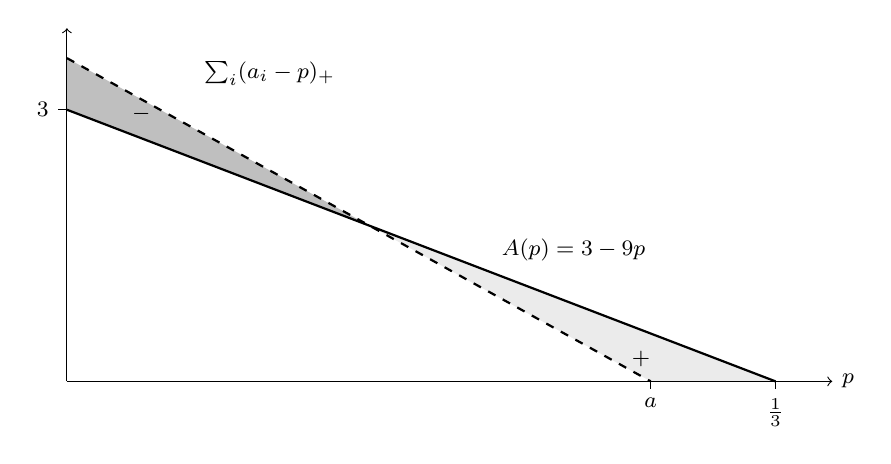
\begin{tikzpicture}[x=27cm,y=1.15cm,font=\footnotesize]
 % deficit and surplus regions for k=13, a=0.99/sqrt(13)=0.2746, h=0.33
 \fill[black!25] (0,3) -- (0,3.570) -- (0.1424,1.718) -- cycle;
 \fill[black!8] (0.1424,1.718) -- (0.2746,0) -- (0.33,0) -- (0.33,0.03) -- cycle;
 \draw[->] (0,0) -- (0.36,0) node[right] {$p$};
 \draw[->] (0,0) -- (0,3.9);
 \draw[thick] (0,3) -- (0.3333,0);
 \draw[thick,dashed] (0,3.570) -- (0.2746,0);
 \draw (0.3333,0) -- (0.3333,-0.08) node[below] {$\tfrac13$};
 \draw (0.2746,0) -- (0.2746,-0.08) node[below] {$a$};
 \draw (0,3) -- (-0.004,3) node[left] {$3$};
 \node[right] at (0.06,3.4) {$\sum_i(a_i-p)_+$};
 \node[right] at (0.2,1.45) {$A(p)=3-9p$};
 \node at (0.035,2.95) {$-$};
 \node at (0.27,0.25) {$+$};
\end{tikzpicture}
\caption{The area profile $A$ of the cubic model (solid) and the slice profile of $13$ balls of capacity
$a=0.99/\sqrt{13}$ (dashed). The deficit (dark) is smaller than the surplus (light), since
$\int_0^h(A-\sum_i(a_i-p)_+)\,dp=\frac12(1-13a^2-(1-3h)^2)>0$ for $h=0.33$, but stacking needs $A\ge\sum_i(a_i-p)_+$
pointwise. The twist moves area from the surplus to the deficit.}
\label{fig:intro-profile}
\end{figure}

\subsection{The twist moves area}\label{sec:mech-twist}

The construction of \cite{OpenAI2026} pays the deficit with the surplus by twisting the bundle: across an annulus in
the base, the fibre over one boundary circle is identified with the fibre over the other by an area-preserving map $q$
of the fibre disc instead of the identity. On the annulus $(s,v)\in[0,1]\times\R/\Z$, let $\beta=b(v)\,dv$ with $b\ge0$ supported in a band and
$\int_0^1b=1$, and let $\nu$ be the base area form. The first Moser path (Section~\ref{sec:hdl}) replaces the model form
on the annulus by $\omega_V+e_h\nu+d(f(s)H^*(p)\beta)$, with background $e_h=g/16$, $H^*=\Hb-e_h$ and a clock $f$
rising from $0$ to $1$; the comparison gap is $\frac{31}{32}g$ and the residual is at least $\frac78g$
(\Sref{Lemma}{lem:shd4-budget}; Table~\ref{tab:mdl-margins}).

Let $q_t$ be the comparator's Hamiltonian isotopy of the fibres, $q=q_1$, and $\mathcal D_\lambda(s,v,w)=(s,v,q_{\lambda f(s)}w)$. For a smooth function $K$ of the moments put $J=K-H^*$; adding $d(J(p)\beta)$ changes only toric mixed terms off the annulus. After the twist, the area available across the annulus at $w$ is
\begin{equation}\label{eq:mech-available}
 K\big(p(q^{-1}w)\big)-J\big(p(w)\big)
 =H^*\big(p(w)\big)+K\big(p(q^{-1}w)\big)-K\big(p(w)\big).
\end{equation}
Since $q$ preserves the fibre area, this redistributes area between moment levels without changing the total. The comparison supplies, for a minorant $P\le\Pb$,
\begin{equation}\label{eq:mech-comparison}
 (K-P)\big(p(qw)\big)\le K\big(p(w)\big)-\gamma\qquad(w\in V_\Delta).
\end{equation}
Integrating over $V_\Delta$ shows that this forces $\int_\Delta P>0$.

The identity \eqref{eq:mech-available} is checked directly. The fibre is $\bar D(h)$, and over the annulus every form is $\omega_V+e_h\nu+d(G\beta)$ with $G(s,w)$ independent of $v$. By Lemma~\ref{lem:hdl-top-power}(b), its restriction to the annulus through $w$ is $e_h\nu+\partial_sG\,ds\wedge\beta$. Hence, beyond the background, the area above $w$ is $G(1,w)-G(0,w)$, which equals $H^*(p(w))$ after the first path. The twist $\mathcal D$ is the identity for $s\le0$ and $(s,v,w)\mapsto(s,v,qw)$ for $s\ge1$. After adding $d(J(p)\beta)$, the coefficient below the annulus is therefore $J(p(w))$. Above it, the coefficient is $H^*(p(z))+J(p(z))=K(p(z))$ at $z=q^{-1}w$, which gives~\eqref{eq:mech-available}.

The \emph{layers} are disjoint subintervals $I_1,\dots,I_k,I_*$ of $(0,1)$ (Figure~\ref{fig:mech-layers}). Across $I_i$ the coefficient rises by a smooth cap $h_i(p(w))$. This cap is an explicit smoothing of $(a_i-p)_+$, above it by at most $\frac g{32}$ in total, and it holds a ball of capacity slightly less than $a_i$ in product form, since the form is toric on $I_i$. Across $I_*$ the coefficient rises by the remainder $R^*(w)$. This remainder is positive because $\gamma$ exceeds the smoothing errors, and it is the only layer coefficient depending on more than $p(w)$.

\begin{figure}[ht]
\centering
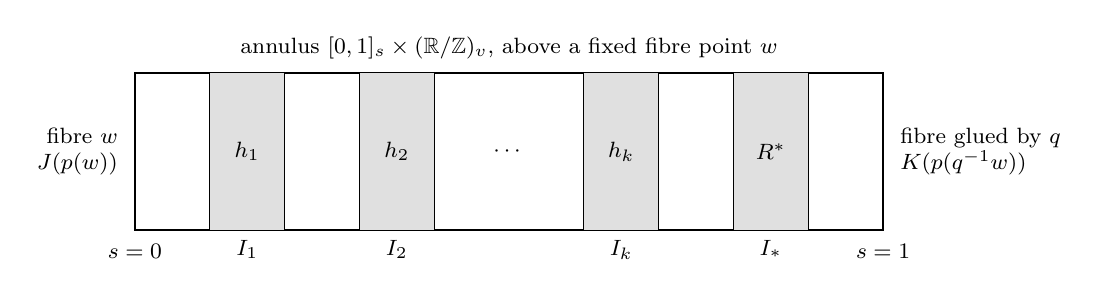
\begin{tikzpicture}[x=0.95cm,y=1cm,font=\footnotesize]
 \draw[thick] (0,0) rectangle (10,2);
 \foreach \l/\r/\t in {1/2/{h_1},3/4/{h_2},6/7/{h_k},8/9/{R^*}} {
  \fill[black!12] (\l,0) rectangle (\r,2);
  \draw (\l,0) -- (\l,2); \draw (\r,0) -- (\r,2);
  \node at ({(\l+\r)/2},1) {$\t$};
 }
 \node at (5,1) {$\cdots$};
 \node[below] at (1.5,0) {$I_1$}; \node[below] at (3.5,0) {$I_2$};
 \node[below] at (6.5,0) {$I_k$}; \node[below] at (8.5,0) {$I_*$};
 \node[below] at (0,-0.05) {$s=0$}; \node[below] at (10,-0.05) {$s=1$};
 \node[left,align=right] at (-0.1,1) {fibre $w$\\$J(p(w))$};
 \node[right,align=left] at (10.1,1) {fibre glued by $q$\\$K(p(q^{-1}w))$};
 \node[above] at (5,2.05) {annulus $[0,1]_s\times(\R/\Z)_v$, above a fixed fibre point $w$};
\end{tikzpicture}
\caption{The annulus above a fibre point $w$ in dimension four. The $\beta$-coefficient rises from $J(p(w))$ to
$K(p(q^{-1}w))$; across the layer $I_i$ it rises by the cap $h_i(p(w))$ of the $i$-th ball and across $I_*$ by the
positive remainder $R^*(w)$.}
\label{fig:mech-layers}
\end{figure}

\subsection{The comparison datum}\label{sec:mech-interfaces}

\begin{definition}[Comparison datum]\label{def:mech-datum}
A comparison datum for $([0,h],P)$ with gap $\gamma>0$ consists of a function $K$, smooth on a neighbourhood of
$[0,h]$, and a smooth Hamiltonian isotopy $(q_t)_{t\in[0,1]}$ of $\C$ with $q_0=\mathrm{id}$, generated by $Q_t$ with
$\iota_{X_{Q_t}}\omega_V=-dQ_t$, such that:
\begin{enumerate}[label=(\arabic*),ref=(\arabic*)]
\item\label{it:mech-datum-collar} $q_t(\bar D(h))=\bar D(h)$ for every $t$, and there is $\varsigma>0$ such that
 $Q_t=0$ on the collar $\{p>h-\varsigma\}$ for every $t$;
\item\label{it:mech-datum-cmp} $q=q_1$ satisfies the comparison inequality~\eqref{eq:mech-comparison}.
\end{enumerate}
\end{definition}

Section~\ref{sec:cmp} constructs the datum in closed form for equal balls with $k\ge10$ and $\frac34<\rho\sqrt k<1$
(Proposition~\ref{prop:cmp-linear}). Comparison data over polytopes, for general concave profiles, are constructed
in~\cite{SongHD}.

\section{Hamiltonian comparison}\label{sec:cmp}

This section produces a comparison datum (Definition~\ref{def:mech-datum}) for the profile of $k\ge10$ equal balls.
Let $h>0$, $\bar D(h)=\{w\in\C:p(w)\le h\}$ with $p=\pi|w|^2$, $\theta=\arg w/2\pi$ and $\omega_V=dp\wedge d\theta$
(\S\ref{sec:mech}), and let $P$ be continuous and concave on $[0,h]$ with positive mean. We seek a smooth $K$ and a
Hamiltonian isotopy $q_t$ of $\bar D(h)$ with $(K-P)\circ p\circ q_1\le K\circ p-\gamma$ for some $\gamma>0$. Since
$p_*\omega_V$ is Lebesgue measure on $[0,h]$, $q_1$ only redistributes the values of $K-P$.

The rearrangement operator is that of \cite[\S2]{OpenAI2026}, where $K$ is the fixed point of a contraction built
from it. For $k\ge10$ equal balls, \S\ref{sec:cmp-linear} gives a closed-form datum with linear $K$ and no fixed
point. Everything is explicit at level L1 (Definition~\ref{def:intro-levels}).

\subsection{The increasing rearrangement}\label{sec:cmp-rearrangement}

\begin{definition}[Increasing rearrangement]\label{def:cmp-rearrangement}
For a continuous convex function $F$ on $[0,h]$ put
\[
 (R_1F)(x)=\min_{0\le a\le h-x}\ \max\bigl(F(a),\,F(a+x)\bigr),\qquad 0\le x\le h .
\]
\end{definition}

The minimum exists, and since sublevel sets of convex functions are intervals, $R_1F$ is the increasing rearrangement
of $F$ on $[0,h]$. The properties used below are in
\Sref{Lemma}{lem:fcp-rearrangement}: $R_1$ is monotone, commutes with adding constants and with multiplication by
$\alpha\ge0$, and preserves integrals and maxima.

\subsection{The linear comparison identity}\label{sec:cmp-linear}

For $k\ge10$ equal capacities in dimension four no fixed point is needed. The height $h=t_0/3$ is chosen so that,
for linear $K$, the function $K-P$ is a constant plus a multiple of a tent that takes the same value at both ends of
$[0,h]$. Each sublevel interval of such a tent has length equal to its level, so its increasing rearrangement is the
identity, and the comparison inequality reduces to a constant gap. This datum serves \Sref{Theorem}{thm:cub-packing}.

Here $\Delta=[0,h]$ with $h$ real (rationality is not used), so $V_\Delta=\bar D(h)$. The symbols $s,a,c_s,g,A,B$ are local to this subsection and to \Ssec{sec:fcp-equal}. For an integer $k\ge10$ and $\eta_\star\in(0,\frac14)$, set $t_0=1-\eta_\star/2$ and
\[
s=\sqrt k,\quad a=\frac{t_0}s,\quad h=\frac{t_0}3,\quad c_s=3s-9,\quad g=3(1-t_0),\quad A=\frac ha,\quad B=\frac h{h-a}.
\]
Since $s>3$, we have $0<a<h$, $c_s>0$, $A,B>0$, and
\begin{equation}\label{eq:cmp-AB}
\frac1A+\frac1B=\frac ah+\frac{h-a}h=1 .
\end{equation}
Let $\Lambda(x)=A(a-x)$ for $x\le a$ and $\Lambda(x)=B(x-a)$ for $x\ge a$. This is a tent with $\Lambda(0)=\Lambda(h)=h$ and $\Lambda(a)=0$.

\begin{lemma}[Sublevel sets of the tent]\label{lem:cmp-tent-sublevel}
\lean{SymplecticPacking.Params.Rcal_le_iff, SymplecticPacking.Params.sublevel_length,
SymplecticPacking.Params.sublevel_subset, SymplecticPacking.Params.volume_sublevel}
\uses{eq:cmp-AB}
For $b\ge0$, $\{x\in\R:\Lambda(x)\le b\}=[a-b/A,\,a+b/B]$, an interval of length $b$. If $b\le h$, it is
contained in $[0,h]$.
\end{lemma}

\begin{proof}
The interval is read off from the two affine pieces. Its length is $b(1/A+1/B)=b$ by \eqref{eq:cmp-AB}. If $b\le h$, then $a-b/A\ge a-h/A=0$ and $a+b/B\le a+h/B=h$.
\end{proof}

\begin{corollary}[Rearrangement of the tent]\label{thm:cmp-tent-rearrangement}
\uses{lem:cmp-tent-sublevel, def:cmp-rearrangement}
On $[0,h]$, $R_1\Lambda(x)=x$ for $0\le x\le h$. Consequently
$R_1(-g+c_s\Lambda)(x)=-g+c_sx$.
\end{corollary}

\begin{proof}
With $\alpha=a-x/A$ we have $\alpha\ge0$, $\alpha+x=a+x/B\le h$ and $\Lambda(\alpha)=\Lambda(\alpha+x)=x$, so $R_1\Lambda(x)\le x$. Conversely, suppose an admissible $[\alpha,\alpha+x]$ had $b'=\max(\Lambda(\alpha),\Lambda(\alpha+x))<x$. By convexity it would lie in $\{\Lambda\le b'\}$, which has length $b'<x$ (Lemma~\ref{lem:cmp-tent-sublevel}); this is impossible. The second claim follows from Lemma~\Snum{lem:fcp-rearrangement}(iv), since $c_s>0$.
\end{proof}

\begin{figure}[ht]
\centering
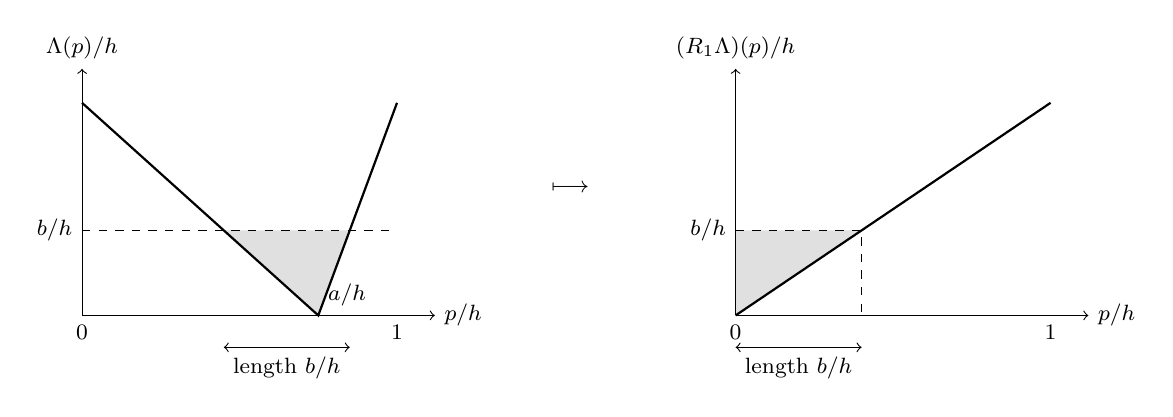
\begin{tikzpicture}[x=4cm,y=2.7cm,font=\footnotesize]
 \begin{scope}
 \fill[black!12] (0.45,0.4) -- (0.75,0) -- (0.85,0.4) -- cycle;
  \draw[->] (0,0) -- (1.12,0) node[right] {$p/h$};
  \draw[->] (0,0) -- (0,1.16) node[above] {$\Lambda(p)/h$};
  \draw[thick] (0,1) -- (0.75,0) -- (1,1);
  \draw[dashed] (0,0.4) node[left] {$b/h$} -- (1,0.4);
  \draw[<->] (0.45,-0.15) -- (0.85,-0.15) node[midway,below] {length $b/h$};
  \node[below] at (0,0) {$0$};
  \node[below] at (1,0) {$1$};
  \node[above right] at (0.75,0) {$a/h$};
 \end{scope}
 \node at (1.55,0.6) {$\longmapsto$};
 \begin{scope}[xshift=8.3cm]
  \fill[black!12] (0,0) -- (0,0.4) -- (0.4,0.4) -- cycle;
  \draw[->] (0,0) -- (1.12,0) node[right] {$p/h$};
  \draw[->] (0,0) -- (0,1.16) node[above] {$(R_1\Lambda)(p)/h$};
  \draw[thick] (0,0) -- (1,1);
  \draw[dashed] (0,0.4) node[left] {$b/h$} -- (0.4,0.4) -- (0.4,0);
  \draw[<->] (0,-0.15) -- (0.4,-0.15) node[midway,below] {length $b/h$};
  \node[below] at (0,0) {$0$};
  \node[below] at (1,0) {$1$};
 \end{scope}
\end{tikzpicture}
\caption{The linear comparison: the sublevel interval of $\Lambda$ has length $b$, so its increasing rearrangement
is $p$. The drawing uses $a/h=3/4$ ($k=16$); the identity holds for every $k\ge10$.
Consequently $K-R_1(K-P)\equiv g$, before the planar realisation error is deducted.}
\label{fig:cmp-tent}
\end{figure}

\begin{proposition}[Linear comparison datum for equal balls]\label{prop:cmp-linear}
\lean{SymplecticPacking.Params.F_eq, SymplecticPacking.Params.margin_one,
SymplecticPacking.Params.K_sub_F_ge, SymplecticPacking.Qhat.K_sub_F_q_ge,
SymplecticPacking.Qhat.full_comparison, SymplecticPacking.Qhat.qhatP_spec,
SymplecticPacking.Branch2.CubicData.ofParams_valid}
\uses{lem:cmp-tent-sublevel, thm:cmp-tent-rearrangement, def:mech-datum, S-lem:fcp-AB, S-def:fcp-eq, S-thm:pll-inner}
With the notation above let $\Delta=[0,h]$, $P(p)=3(1-3p)-k(a-p)_+$, $K(p)=c_sp$ and $F=K-P$. Then
\begin{equation}\label{eq:cmp-identity}
 F(x)=-g+c_s\Lambda(x)\qquad(x\in\R).
\end{equation}
Let $e_q=\min\bigl(h/100,\ g/(128c_s)\bigr)$ (\Sref{Definition}{def:fcp-eq}) and let $(q_t)$ be the isotopy of
\Sref{Theorem}{thm:pll-inner}, whose endpoint $q=q_1$ satisfies $\Lambda(p(q(z)))\le\pi|z|^2+4e_q$ on $\bar D(h)$.
Then $(K,(q_t))$ is a comparison datum for $(\Delta,P)$ with gap $\tfrac{31}{32}g$.
\end{proposition}

\begin{proof}
By \Sref{Lemma}{lem:fcp-AB}, $c_sA=k-3s$, $c_sB=3s$ and $3sa=3-g$. Hence both sides of \eqref{eq:cmp-identity} equal $(3s-k)x+ka-3$ for $x\le a$, and $3sx-3$ for $x\ge a$.

By \Sref{Theorem}{thm:pll-inner}, $q_0=\mathrm{id}$ and each $q_t$ maps $\bar D(h)$ onto itself. Moreover $q_t=\mathrm{id}$ and $Q_t=0$ on $\{\pi|z|^2>P_{\rm supp}\}$ for a constant $P_{\rm supp}<h$; this gives condition~\ref{it:mech-datum-collar} of Definition~\ref{def:mech-datum}.

For condition~\ref{it:mech-datum-cmp}, let $w\in\bar D(h)$ and $I=p(w)$. By \eqref{eq:cmp-identity} and $4c_se_q\le g/32$,
\[
K(I)-(K-P)\bigl(p(q(w))\bigr)=c_sI+g-c_s\Lambda\bigl(p(q(w))\bigr)\ge g-4c_se_q\ge\tfrac{31}{32}g .\qedhere
\]
\end{proof}

Thus $K-R_1F\equiv g$ exactly (Corollary~\ref{thm:cmp-tent-rearrangement}), and the planar map costs at most $g/32$. Ideally $q$ would carry each centred disc $\bar D(b)$, $0\le b\le h$, onto the sublevel set
$\{\Lambda\circ p\le b\}=\{a-b/A\le p\le a+b/B\}$, an annulus (a disc for $b=h$) of the same area $b$, nested in $b$; no
area-preserving homeomorphism does this exactly (\Ssec{sec:fcp-equal}). The map of \Sref{Theorem}{thm:pll-inner} is
built from Morse charts of a smoothed tent potential. On the core $\bar D(h-\frac{31}8e_q)$ its error is below
$\frac{13}{24}e_q$; the full loss $4e_q$ occurs only on the outer annulus, where $q$ is joined to the identity.
In \cite{OpenAI2026} the comparison function is the fixed point of the contraction $T_\lambda$ and the gap comes from
the contraction argument; here the identity~\eqref{eq:cmp-identity} gives it directly. As $t_0\to1$, $g\to0$ while
$ka^2=t_0^2\to1$. The equal-capacity branch takes $\eta_\star=1-\rho\sqrt k$, so $t_0=(1+\rho\sqrt k)/2$ and
$g=3\eta_\star/2$.

\begin{remark}[The range of the linear datum]\label{rem:cmp-small-k}
The linear comparison is used when the capacities are equal, $k\ge10$ and $\eta_\star=1-\rho\sqrt k$ lies in
$(0,\frac14)$, that is $\frac34<\rho\sqrt k<1$. For $k=9$ the formulas give $a=h$, and for unequal capacities a
linear $K$ can fail; these inputs use the scalar comparison datum of the companion paper~\cite{SongHD}.
\end{remark}

\section{Packing over a handle}\label{sec:hdl}

The handle construction is an explicit version of the surface packing lemma of \cite[\S3.2]{OpenAI2026}, with the
Moser argument \cite{Moser1965} carried out by explicit vector fields. We describe it for the cubic model; the
higher-dimensional version is in \cite{SongHD}.

\emph{Setting.} The base is the torus $\Gamma$, and we work on the cover $\R^2\times\C$ with coordinates $(u,v,w)$,
$p=\pi|w|^2$, equivariantly under the deck maps, which shift $(u,v)$ by integers and preserve $p$
(\Sref{Definition}{def:cub-model}). The \emph{marked fibres} are the fibres over the three points of $\Gamma$ where
$Z_0=0$. The handle data (\Sref{Proposition}{prop:cub-handle}) are an annulus
$\mathcal A=\{\frac18\le u\le\frac5{24}\}\subset\mathcal A^+=\{\frac1{12}\le u\le\frac14\}$, which misses the marked
points, with handle coordinate $s=12u-\frac32\in[0,1]$; the area form $\nu=du\wedge dv$; and the closed one-form
$\beta=b(v)\,dv$ with $b\ge0$ supported in a band and $\int_0^1b=1$. Over $\mathcal A^+$ the bundle is trivialised by the
frame chart $\chi_{\mathcal A}(u,v,w_{\mathcal A})=(u,v,(Z_0/|Z_0|)^3w_{\mathcal A})$ (\Sref{Definition}{def:shd4-frame}).
The data $h,g,K,(q_t)$ are valid cubic data (\Sref{Definition}{def:shd4-data}): in the linear branch, those of
Proposition~\ref{prop:cmp-linear}.

\emph{The three paths.} All three are exact paths of deck-invariant forms with explicit primitives.
\begin{enumerate}[label=(\arabic*)]
\item The \emph{first path} $\Omega_t=\Omega_0+t\,d\alpha_1$, with the closed-form primitive $\alpha_1$ of
 \Sref{Construction}{cons:fer-alpha1}, moves the usable base area onto the annulus: over $\mathcal A$,
 $\chi_{\mathcal A}^*\Omega_1=\omega_V+e_h\nu+d\bigl(f(u)H^*(p)\beta\bigr)$ with $e_h=g/16$, $H^*=\Hb-e_h$ and the clock
 $f$, which rises from $0$ to $1$ inside $\mathcal A$ (\Sref{Lemma}{lem:shd4-frame-forms}).
\item The \emph{second path} inserts the comparator isotopy across the annulus by the twist below
 (\Sref{Proposition}{prop:shd4-second}).
\item The \emph{third path} separates the caps $h_i$ of the balls into disjoint layers in the $u$-direction, with a
 positive residual layer (\Sref{Proposition}{prop:shd4-third}).
\end{enumerate}
The Moser flow of the concatenated path is the handle Moser map $\Phi$, and the layer maps $E_i$ place the balls in
the layers (Remark~\ref{rem:hdl-four}).

\subsection{The twist}\label{sec:hdl-twist}

The two computations behind the second path hold for fibres $\C^m$ of any rank $m$; we state them in that generality
because the companion paper~\cite{SongHD} uses them for $m\ge2$. Here $m=1$, $n=2$, $\omega_V=\sum_jdp_j\wedge d\theta_j$ is the fibre form, and the handle coordinates are $(s,v)$.
A \emph{horizontal} one-form annihilates fibre tangent vectors.

\begin{lemma}[Top power]\label{lem:hdl-top-power}
\lean{SymplecticPacking.Forms.pf_splitForm,
SymplecticPacking.Handle.Cubic.OmegaPreG_split,
OAI.PackingSufficiencySupport.Hamiltonian.toric_horizontalCoupling_isInvertible,
OAI.PackingSufficiencySupport.Hamiltonian.oneCovectorForm_isInvertible}
\begin{enumerate}[label=(\alph*)]
\item In local product coordinates let $\kappa'$ be a base two-form and $a'_1,\dots,a'_m$ base one-forms, with
coefficients depending on the base point and on $p$. Then
$(\omega_V+\kappa'+\sum_jdp_j\wedge a'_j)^n=n\,\omega_V^m\wedge\kappa'$.
\item On $\mathcal A^+\times\C^m$, in product coordinates, let $\sigma_{\mathcal A}=a_{\mathcal A}(s,v)\,ds\wedge dv$ be a positive area form on the annulus, let $G(s,w)$ be smooth and
independent of $v$, and $e>0$. Then
$\big(\omega_V+e\sigma_{\mathcal A}+d(G\beta)\big)^n=n\,(e a_{\mathcal A}(s,v)+b(v)\,\partial_sG)\,\omega_V^m\wedge ds\wedge dv$.
\end{enumerate}
In particular the forms in (a) are nondegenerate where $\kappa'>0$; when closed, they are
symplectic there. The forms in (b) are symplectic where $\partial_sG\ge0$.
\end{lemma}

\begin{proof}
Let $x_j,y_j$ be the fibre covectors and $\sigma,\tau$ the base covectors at a point. Then $dp_j=u_jx_j+v_jy_j$ and $a'_j=A_j\sigma+B_j\tau$, and $x_j\wedge y_j+dp_j\wedge a'_j=(x_j-v_ja'_j)\wedge(y_j+u_ja'_j)$, so each block is decomposable. The blocks commute and square to zero, so the $m$-th power of their sum is $m!$ times their product. Every base correction in that product vanishes against the base area. Adding $\kappa'$ then gives (a), including where a moment differential vanishes. For (b), the mixed part of $d(G\beta)=\partial_sG\,ds\wedge\beta+d_wG\wedge\beta$ is fibre-covector${}\wedge\beta$. The same factorization therefore gives $n\omega_V^m\wedge(e\sigma_{\mathcal A}+\partial_sG\,ds\wedge\beta)$, with $\beta=b(v)\,dv$. Positive coefficients give a nonzero top power.
\end{proof}


Let $(q_t)$ be the comparator isotopy, generated by $Q_t$ with $\iota_{X_{Q_t}}\omega_V=-dQ_t$, and $q=q_1$; in dimension
four $q_t$ is the identity on $\{p>P_{\rm supp}\}$ with $P_{\rm supp}<h$, so it preserves the fibre disc $\bar D(h)$.
Let $f$ be a clock, $f=0$ for $s\le0$ and $f=1$ for $s\ge1$, and let $H^*$ be a function of the moments. For
$\lambda\in[0,1]$ define on $\mathcal A\times\C^m$
\begin{equation}\label{eq:hdl-twist}
 \mathcal D_\lambda(s,v,w)=\big(s,v,q_{\lambda f(s)}(w)\big),\qquad
 Q^\lambda_s=\lambda f'(s)\,Q_{\lambda f(s)},\qquad
 G_\lambda(s,w)=f(s)\,H^*\big(p(q_\lambda^{-1}(w))\big),
\end{equation}
and $\mathcal D=\mathcal D_1$. Then $\partial_sq_{\lambda f(s)}=X_{Q^\lambda_s}\circ q_{\lambda f(s)}$. The twist changes
the fibre identification across the annulus from the identity to $q$.

\begin{lemma}[Suspension]\label{lem:hdl-suspension}
\lean{SymplecticPacking.HighDim.RawModelAgreement.firstPath_semantic, SymplecticPacking.Handle.Cubic.suspension, SymplecticPacking.Handle.Cubic.eta_support}
\uses{def:mech-datum, S-lem:shd4-frame-forms}
Let $\sigma_0$ be a base two-form on $\mathcal A$. On $\mathcal A\times\C^m$, for $\lambda\in[0,1]$:
\begin{enumerate}[label=(\roman*)]
\item $\mathcal D_\lambda^*\omega_V=\omega_V+d\big[(Q^\lambda_s\circ q_{\lambda f(s)})\,ds\big]$;
\item with the horizontal one-form
\[
 \eta_\lambda=(Q^\lambda_s\circ q_{\lambda f(s)})\,ds
 +f(s)\Big[H^*\big(p(q_\lambda^{-1}q_{\lambda f(s)}(w))\big)-H^*\big(p(w)\big)\Big]\beta ,
\]
one has
$\mathcal D_\lambda^*\big(\omega_V+\sigma_0+d(G_\lambda\beta)\big)=\omega_V+\sigma_0+d\big(f(s)H^*(p)\beta\big)+d\eta_\lambda$;
\item $\eta_0=0$, $\eta_\lambda$ is smooth in $(\lambda,s,v,w)$, and $\eta_\lambda=0$ for $s\notin(0,1)$, so it extends
by zero to a horizontal one-form supported over $\mathcal A$. If the first path ends at a form $\Omega_1$ equal to
$\omega_V+\sigma_0+d(f(s)H^*(p)\beta)$ over $\mathcal A$ (\Sref{Lemma}{lem:shd4-frame-forms} for $n=2$; for $n\ge3$
see~\cite{SongHD}), then
$\Omega_1+d\eta_\lambda=\mathcal D_\lambda^*\big(\omega_V+\sigma_0+d(G_\lambda\beta)\big)$ over $\mathcal A$.
\end{enumerate}
\end{lemma}

\begin{proof}
(i) Put $\Theta(s,w)=Q^\lambda_s(q_{\lambda f(s)}(w))$ and $q=q_{\lambda f(s)}$; the right side is $\omega_V+d_w\Theta\wedge ds$. The map $d\mathcal D_\lambda$ fixes $\partial_v$, sends a vertical $u$ to $Dq\,u$, and sends $\partial_s$ to $\partial_s+X_{Q^\lambda_s}(q(w))$. Since $q$ is symplectic, both sides agree on vertical pairs. On $(\partial_s,u)$ the left side is $\omega_V(X_{Q^\lambda_s},Dq\,u)=-d_w\Theta(u)$. Pairs involving $\partial_v$ vanish on both sides.
(ii) $\mathcal D_\lambda$ fixes base points, so it preserves $\sigma_0$ and $\beta$. Moreover $\mathcal D_\lambda^*(G_\lambda\beta)=f(s)H^*(p(q_\lambda^{-1}q_{\lambda f(s)}w))\beta$; add (i).
(iii) For $s\le0$, $f=f'=0$. For $s\ge1$, $f=1$, $f'=0$ and $q_\lambda^{-1}q_{\lambda f(s)}=\mathrm{id}$. The last identity is (ii) with the assumed form of $\Omega_1$.
\end{proof}

Using the fixed map $q_\lambda^{-1}$ in $G_\lambda$ makes the bracket vanish identically for $s\ge1$, and it gives $\partial_sG_\lambda=f'(s)H^*(p(q_\lambda^{-1}w))$.

\emph{The second path.} Put $\Omega^{(1)}_\lambda=\Omega_1+d\eta_\lambda$; it equals $\Omega_1$ off the annulus. Over the
annulus it is $\mathcal D_\lambda^*$ of a form whose top power is, by Lemma~\ref{lem:hdl-top-power}(b) with $n=2$,
$\sigma_0=e_h\nu$, $2\bigl(e_h+b(v)f'(u)H^*(p(q_\lambda^{-1}w))\bigr)\,\omega_V\wedge du\wedge dv$, positive on
$\{p<h+2\delta_m\}$ because $H^*>0$ there. Since $\mathcal D_\lambda$ preserves orientation, $\Omega^{(1)}_\lambda$ is an
exact symplectic path on this region (\Sref{Proposition}{prop:shd4-second}). Only the forms, not $\mathcal D_\lambda$,
are glued to the model. The higher-dimensional handle and the packing theorem in a toric model are in the companion
paper~\cite{SongHD}.

\begin{remark}[Dimension four]\label{rem:hdl-four}
For $n=2$ the construction is carried out on the cover, equivariantly under the deck maps, (\Ssec{sec:shd-four}). The clock is $f(u)=S((u-\frac7{48})/\frac1{24})$, i.e.\ $S(2s-\frac12)$, and the $k+1$ layer
intervals lie inside its ramp. The caps are $h_i(p)=\frac12\bigl(a_i-p+\sqrt{(a_i-p)^2+\mu_h^2}\bigr)$ with
$\mu_h=g/(16k)$; they lie above the tents and exceed them in total by at most $g/32$, so a comparison gap
$\frac{31}{32}g$ leaves a residual of at least $\frac78g$. The three paths are concatenated into one flow, cut off only
in the moment variable, on $\{p<h+2\delta_m\}$, $\delta_m=\min((d_n-h)/4,g/100)$. All three variation primitives vanish
as covectors on the marked fibres, so the flow fixes them pointwise and the images avoid $\{Z_0=0\}$
(\Sref{Lemma}{lem:shd4-fibres}, \Sref{Propositions}{prop:shd4-moser} and~\Snum{prop:shd4-maps}).
\end{remark}


\section{The four-dimensional model and the return to the ball}\label{sec:mdl}

This section describes the four-dimensional model, the return to the ball and the margins of the construction;
details are in \Ssec{sec:cub} and \Ssec{sec:rtc}. Throughout, the target is $\Bo(1)$ and $\rho_i=c_i/C$.

\subsection{The cubic model}\label{sec:mdl-cub}

The model is the normal disc bundle of Biran's decomposition of $\CP^2$ along a smooth cubic \cite{Biran2001}, written on the cover $\R^2\times\C$ of the Fermat torus $\Gamma=\C/(\Z+\zeta\Z)$, $\zeta=e^{2\pi i/3}$. Theta functions give a smooth map $Z\colon\R^2\to\C^3$, periodic up to phase, with $|Z|=1$ and $Z_0^3+Z_1^3+Z_2^3=0$. With $\eta_\Gamma=\frac1{2\pi}\operatorname{Im}\sum_j\overline{Z_j}\,dZ_j$, $\sigma=d\eta_\Gamma$ and $p=\pi|w|^2$, the model form is
\[
 \Omega_0=\omega_V+(1-3p)\,\sigma-3\,dp\wedge\eta_\Gamma ,\qquad \int_\Gamma\sigma=3,
\]
so the base area at level $p$ is $3(1-3p)$, the fibre interval stops below $p=\frac13$, and hence $3c_i<C$. The integrated profile over $[0,h]$ is $3h-\frac92h^2\to\frac12=\vol\CP^2$ as $h\uparrow\frac13$ (\Sref{Lemma}{lem:cub-volume}).

\begin{theorem}[Packing in dimension four]\label{thm:mdl-cub}
Let $(k,\rho_i,a_i,h,d_n,g,K,q)$ be valid cubic data (\Sref{Definition}{def:shd4-data}) with $d_n=\frac12(h+\frac13)$:
$0<\rho_i<a_i<h<d_n<\frac13$, $0<g\le3(1-3h)$, and $(K,(q_t))$ a comparison datum for the profile
$3(1-3p)-\sum_i(a_i-p)_+$ on $[0,h]$ with gap $\frac{31}{32}g$, whose isotopy is the identity near $p=h$. Then there are
explicit numbers $\rho_i<\rho_i^+<\rho_i^{\rm dom}$ and smooth maps $f_i\colon\Bo(\rho_i^{\rm dom})\to\C^2$ with symplectic
derivative, injective on $B(\rho_i^+)$, such that the sets $f_i(B(\rho_i^+))$ are pairwise disjoint and contained in
$B(1-\mu_{\rm ball})$ for some $\mu_{\rm ball}\in(0,1)$.
\end{theorem}

This is \Sref{Theorem}{thm:cub-packing}. For $k\ge10$ equal capacities with $\frac34<\rho\sqrt k<1$ the data are
given by the linear datum of Proposition~\ref{prop:cmp-linear}, with $a=t_0/\sqrt k$, $h=t_0/3$,
$t_0=(1+\rho\sqrt k)/2$, all algebraic in $\sqrt k$ and $\rho$ (\Sref{Remark}{rem:cub-lean}). For all other
$\rho_i<\frac13$ with $\sum_i\rho_i^2<1$, including $k=9$ and unequal capacities, the companion paper~\cite{SongHD}
constructs valid cubic data from a scalar comparison datum. The embeddings are
\[
 f_i=b_{\rm ball}\circ\psi_1^{-1}\circ\mathrm{pr}\circ\tau_1\circ\iota\circ\mathsf N\circ\Phi^{-1}\circ\chi_{\mathcal A}
 \circ\mathcal D^{-1}\circ E_i ,
\]
read from right to left as follows. The layer map $E_i$, built from an explicit strip map and a unique root, places the
ball in the $i$-th layer over the annulus (\Sref{Proposition}{prop:shd4-maps}); $\mathcal D$ is the twist and
$\chi_{\mathcal A}$ the frame chart over the annulus (Section~\ref{sec:hdl}); $\Phi$ is the handle Moser map, which
commutes with the deck maps and fixes the marked fibres (Remark~\ref{rem:hdl-four}); $\mathsf N(u,v,w)=(Z(u,v),w)$
passes from the cover to unit Fermat representatives; and $\iota,\tau_1,\mathrm{pr},\psi_1^{-1},b_{\rm ball}$ form the
return of \S\ref{sec:mdl-return}. The argument
is outlined in \Ssec{sec:mdl-cub-outline}.

\subsection{The return to the ball}\label{sec:mdl-return}

The handle maps land in $\{p<h\}$ of the model on the cover, and the return carries this region into
$\CP^2\setminus\{Z_0=0\}$, which the affine chart $b_{\rm ball}$ identifies with $\Bo(1)$. It is a deformation to the
normal cone, following the scheme of \cite{OpenAI2026}, written with explicit flows
(\Sref{Construction}{cons:cub-transfer}). Let $\mathcal F(Z)=Z_0^3+Z_1^3+Z_2^3$ and $X_T=\{\mathcal F(Z)=TW\}$, with $W$ of
weight three: $X_0$ is the total space of $\mathcal O(3)|_E$ over the cubic, and $X_1$ is a graph over $\CP^2$. The
return is $\mathcal T=b_{\rm ball}\circ\psi_1^{-1}\circ\mathrm{pr}\circ\tau_1\circ\iota\circ\mathsf N$: $\mathsf N$ passes to
unit Fermat representatives, $\iota$ is an explicit weight-three injection into $X_0$, $\tau_1$ is the time-one map of
an explicit transport field from $X_0$ to $X_1$ preserving the restricted forms, $\mathrm{pr}$ is the projection of the
graph, and $\psi_1^{-1}$ is the inverse of an explicit Moser return removing an exact term from the Fubini--Study form.
The denominators of both fields are bounded below on the regions the trajectories visit (Table~\ref{tab:mdl-margins}).
Then $\mathcal T$ pulls $\omega_0$ back to $\Omega_0$ on $\{p<h\}$ off the marked fibres and identifies exactly
deck-equivalent points (\Sref{Theorem}{thm:rtc-transfer}).

The images must avoid the line $L=\{Z_0=0\}$, which the ball chart removes. This follows from a symmetry. Let
$\mathsf r(Z,W)=(\zeta Z_0,Z_1,Z_2,W)$.
\begin{enumerate}[label=(\alph*)]
\item $\mathsf r$ is unitary and preserves $\mathcal F$, so it preserves the forms and constraints above; since
 $\bar\zeta^2=\zeta$ it maps both fields to themselves. Hence $\iota$, $\tau_1$, $\mathrm{pr}$ and $\psi_1^{-1}$ commute with
 $\mathsf r$ (\Sref{Lemma}{lem:rtc-equivariant}).
\item Each factor is injective on representatives and commutes with the gauge action $(Z,W)\mapsto(cZ,c^3W)$, so
 $\mathcal T_{\rm u}=\psi_1^{-1}\circ\mathrm{pr}\circ\tau_1\circ\iota$ is injective modulo gauge
 (\Sref{Lemma}{lem:rtc-injective}).
\item For a point $x=(Z,U)$ of the central fibre, $\mathsf rx$ is a gauge multiple of $x$ only if $Z_0=0$
 (\Sref{Lemma}{lem:rtc-fixed}).
\end{enumerate}
If an output $Y=\mathcal T_{\rm u}(x)$ had $Y_0=0$, then $\mathsf rY=Y$, so by (a) and (b) $\mathsf rx$ is a gauge multiple
of $x$, and (c) gives $Z_0=0$. The handle construction
keeps the balls off the marked fibres, the fibres over the points of $E$ with $Z_0=0$: the layers lie over the
annulus, which misses these points, and the three Moser flows fix the marked fibres pointwise because their variation
primitives vanish there (\Sref{Lemma}{lem:shd4-fibres}). Hence the images avoid $L$, with a positive margin
$\mu_{\rm ball}$ to $\partial\Bo(1)$ on every compact family (\Sref{Proposition}{prop:rtc-avoid}).

\subsection{Margins}\label{sec:mdl-margins}

Each step of the construction leaves a quantitative margin that a later step consumes; Table~\ref{tab:mdl-margins}
lists them for the linear branch. The gap $g=3(1-t_0)=\frac32\eta_\star$ pays for the planar cost ($\le\frac g{32}$),
the background $e_h=\frac g{16}$ and the cap excess ($\le\frac g{32}$), leaving a residual of at least $\frac78g$.

\begin{table}[!htbp]
\centering\footnotesize
\renewcommand{\arraystretch}{1.15}
\begin{tabular}{@{}L{0.2\textwidth}L{0.29\textwidth}L{0.27\textwidth}L{0.17\textwidth}@{}}
\toprule
Margin & Definition; dependence & Used for & Source\\
\midrule
volume defect & $\eta_\star=1-\rho\sqrt k$; input & $\eta_\star=(1-t_0)+\sqrt k(a-\rho)$, $\frac{\eta_\star}2$ each & hypothesis\\
capacity slack $a-\rho$ & $\frac{\eta_\star}{2\sqrt k}$ & half to $\bar\rho$; strip excess $\frac{\delta}2$; $\frac{\delta}4$ left below $h_i$ & Rem.~\Snum{rem:rtc-equal}\\
ball enlargement $\rho<\rho^+<\rho^{\rm dom}$ & $(\rho \varrho_3^2,\rho \varrho_4^2)$; $\rho$, $a$ & closed source $B(\rho^+)$, open domain $\Bo(\rho^{\rm dom})$ & Rem.~\Snum{rem:rtc-recorded}, Prop.~\Snum{prop:shd4-maps}\\
fibre height $1-3h$ & $1-t_0=\frac{\eta_\star}2$ & $g\le\Hb(h)=3(1-3h)$; transfer margins & Rem.~\Snum{rem:rtc-equal}\\
gap $g$ & $3(1-t_0)$ & all handle margins below & Prop.~\ref{prop:cmp-linear}\\
planar tolerance $e_q$ & $\min(\frac h{100},\frac g{128c_s})$ & $\Lambda(p(q(z)))\le\pi|z|^2+4e_q$; cost $4c_se_q\le\frac g{32}$ & Def.~\Snum{def:fcp-eq}, Thm.~\Snum{thm:pll-inner}, Lem.~\Snum{lem:fcp-margin}\\
comparison gap $\ge\frac{31}{32}g$ & $g$ minus the planar cost & background, cap excess, residual & Prop.~\ref{prop:cmp-linear}\\
background $e_h=\frac g{16}$ & $H^*=\Hb-e_h\ge\frac{15}{16}g$ on $[0,h]$ & positive form $e_h\,du\wedge dv$ on the annulus & Rem.~\ref{rem:hdl-four}, Lem.~\Snum{lem:shd4-budget}(b)\\
cap width $\mu_h=\frac g{16k}$ & $h_i=\frac12(a_i-p+\sqrt{(a_i-p)^2+\mu_h^2})$ & cap excess $\sum_i(h_i-(a_i-p)_+)\le\frac g{32}$ & Rem.~\ref{rem:hdl-four}, Lem.~\Snum{lem:shd4-budget}(a)\\
residual $\frac78g$ & $\frac{31}{32}g-e_h-\frac g{32}$ & positive remainder layer $R^*$ & Lem.~\Snum{lem:shd4-budget}(c)\\
planar support $h-P_{\rm supp}$ & isotopy data of Def.~\Snum{def:pln-isotopy-data}; $P_{\rm supp}>h-\frac{31}8e_q$ & all flows preserve $p$ above $P_{\rm supp}$ & Lem.~\Snum{lem:pln-data}, positivity\\
safe region $\{p<h+2\delta_m\}$ & $\delta_m=\min(\frac{d_n-h}4,\frac g{100})$; cutoff on $[h+\frac32\delta_m,h+\frac74\delta_m]$ & $H^*>\frac{15}{16}g-18\delta_m$; Moser identity on $\{p\le h+\delta_m\}$ & Lem.~\Snum{lem:shd4-budget}(d)\\
base speed $C_b$ & maximum over a compact fundamental set & completeness of the handle flow & positivity only\\
transfer margins & $d_n-h=\frac12(\frac13-h)$, $1-3d_n=\frac12(1-3h)$; $h$ & $\iota$ needs $p<d_n$; $A>1-3d_n$; $w_*=\frac h{d_n-h}$ & explicit\\
transport denominator & $N_{\rm den}\ge c_*=\min(\frac32,\frac{T_0^2}{d_n})$; $d_n$, $w_*$ & cutoff at $\frac{c_*}2$, inactive on $\mathcal C_*$ & Lem.~\Snum{lem:rtc-denominator}\\
return denominator & $A_s+B_sG\ge1-\frac32d_n>\frac12$; $d_n$ & cutoff at half the bound, inactive & Lem.~\Snum{lem:rtc-graph}\\
target boundary $\mu_{\rm ball}$ & $\frac12\min_{\mathcal K}(1-\pi|z|^2)=\frac12\min|Y_0|^2$ & compactness of $\bigcup_if_i(B(c'_i))\subset\Bo(C)$ & Prop.~\Snum{prop:rtc-avoid}, positivity only\\
radii $r_i<r_{1,i}<\dots<r_{4,i}<r'_i$ & $r_{\ell,i}=r_i+\frac\ell5\min(\frac14\text{centre gap},r'_i-r_i)$ & cutoff collar, disjoint closed balls, open domain & Lem.~\ref{lem:ham-radii}\\
isotopy scale $\tau$ & $\min(\frac12,\frac{\delta_c}{2Lr_{\rm tot}})$; $L$ a maximum over compact sets & separation $|Y_i-Y_j|\ge4Lr_{\rm tot}$ & Lem.~\Snum{lem:iso-parameters}, positivity only\\
\bottomrule
\end{tabular}
\caption{Margins of the construction in the linear branch, in the order in which they are used. The table is an
index into the supplement: symbols not defined in the main text are defined at the cited statements. ``Explicit''
means that the margin is a closed formula in the inputs; ``positivity only'' means that the proof shows the number is
positive without bounding it.}
\label{tab:mdl-margins}
\end{table}

\emph{A worked instance.} \Ssec{sec:example} takes $k=10$, $\eps=\frac1{10}$ in Theorem~\ref{thm:intro-4d}:
$R=(k/(1-\eps/4))^{1/4}$, $C=\pi R^2$, $c_i=\pi$, $s_i=(3i-3,0,0,0)$, so $\rho=\sqrt{39}/20$,
$\rho\sqrt k=\sqrt{39/40}\in(\frac34,1)$ and the linear datum applies, with $K(p)=(3\sqrt{10}-9)p$; the supplement lists
the resulting constants and margins and the composed Hamiltonian.

\section{From embeddings to one Hamiltonian; proof of Theorem~\texorpdfstring{\ref{thm:intro-4d}}{A}}\label{sec:ham}

We join the translations $u\mapsto s_i+u$ to the embeddings $f_i$ of Section~\ref{sec:mdl} by one explicit family $F_{i,t}$ of symplectic embeddings with pairwise disjoint images at every time (\S\ref{sec:ham-isotopy}). We then write down a Hamiltonian on $\R\times\R^{2n}$ whose field is the velocity of this family on the moving balls (\S\ref{sec:ham-hamiltonian}). Every stage is a formula, an integral, a matrix function, a maximum over a compact set, a definite description, or the least of finitely many angle indices.

\emph{Notation.} $\EB(y,r)$ and $\EB^\circ(y,r)$ are the closed and open Euclidean balls of radius $r$ about $y\in\R^{2n}$, with $\EB(r)=\EB(0,r)$; thus $B(s,c)=\EB(s,\sqrt{c/\pi})$. We write $\omega_0(v,w)=v^{\mathsf T}J_0w$ with $J_0=\left(\begin{smallmatrix}0&I\\-I&0\end{smallmatrix}\right)$ in coordinates $(x,y)$, so $X_H=J_0\nabla H$ and $\iota_{X_H}\omega_0=dH$. Multiplication by $i$ on $\C^n$, $z_j=x_j+iy_j$, is $J_\C=-J_0$. $\operatorname{Sp}(2n)=\{A:A^{\mathsf T}J_0A=J_0\}$, and $\|\cdot\|$ is the Euclidean operator norm.

Two observations drive the construction: the maps $u\mapsto v^{-1}f_i(vu)$, $0<v\le1$, are symplectic with disjoint images for a common $v$; and on the source ball the one-form $\omega_0(\dot F,DF\,\cdot)$ is closed, with an explicit radial primitive.

\subsection{The embeddings}\label{sec:ham-embeddings}

\begin{definition}[Normalisation]\label{def:ham-normalise}
Let $C>0$ and $c\in(0,\infty)^k$. The \emph{normalised capacities} are $\rho_i=c_i/C$. For a map $f^\natural$
defined on a subset of $\R^{2n}$, its \emph{physical rescaling} is $f(u)=\sqrt C\,f^\natural(u/\sqrt C)$.
\end{definition}

The dilation $\delta(z)=z/\sqrt C$ maps $B(s,c)$ onto $B(s/\sqrt C,c/C)$ and $\Bo(C)$ onto $\Bo(1)$. Definition~\ref{def:intro-admissible} is homogeneous, so $(n,k,C,c)$ is admissible iff $(n,k,1,\rho)$ is. Moreover $f=\delta^{-1}\circ f^\natural\circ\delta$ has $Df(u)=Df^\natural(u/\sqrt C)$, so it is symplectic, injective or of disjoint images exactly when $f^\natural$ is.

In the \emph{linear branch}, $n=2$, $k\ge10$, equal normalised capacities $\rho_i=\rho$ and $\frac34<\rho\sqrt k<1$,
\Sref{Construction}{cons:ham-branch} defines \emph{normalised embeddings} $f^\natural_i$, an enlarged closed capacity
$\rho_i^+$ and an open domain capacity $\rho_i^{\rm dom}$, with $\rho_i<\rho_i^+<\rho_i^{\rm dom}$, from the cubic model
with the linear datum. These capacities are closed formulas in $\rho$ built from arithmetic and square roots. The
constructions of this section other than the embeddings hold in every dimension.

\begin{definition}[Embedding datum]\label{def:ham-datum}
\lean{SymplecticPacking.General.EmbeddingData, SymplecticPacking.General.EmbeddingSpec}
Let $n\ge1$, $k\ge1$, $C>0$ and $c\in(0,\infty)^k$. An \emph{embedding datum} for $(n,k,C,c)$ consists of numbers
$c'_i,\bar c_i$ with $c_i<c'_i<\bar c_i$ and maps $f_i\colon\Bo(\bar c_i)\to\R^{2n}$ such that
\begin{enumerate}[label=(\roman*)]
\item $f_i$ is $C^\infty$ and $Df_i(u)\in\operatorname{Sp}(2n)$ for all $u\in\Bo(\bar c_i)$;
\item $f_i$ is injective on $B(c'_i)$;
\item the sets $f_i(B(c'_i))$, $1\le i\le k$, are pairwise disjoint and contained in $\Bo(C)$.
\end{enumerate}
\end{definition}

\begin{proposition}[The embeddings]\label{prop:ham-embeddings}
\uses{cons:ham-branch, S-thm:cub-packing}
Let $k\ge10$, $C>0$ and $c_1=\dots=c_k=c>0$ with $\rho=c/C$ in the linear branch, $\frac34<\rho\sqrt k<1$, and let
$f^\natural_i$, $\rho_i^+$ and $\rho_i^{\rm dom}$ be given by \Sref{Construction}{cons:ham-branch}. Put
\[
 c'_i=C\rho_i^+,\qquad \bar c_i=C\rho_i^{\rm dom},\qquad f_i(u)=\sqrt C\,f^\natural_i(u/\sqrt C).
\]
Then $(c'_i,\bar c_i,f_i)$ is an embedding datum for $(2,k,C,c)$, and $\bigcup_if_i(B(c'_i))$ is a compact subset of
$\Bo(C)$.
\end{proposition}

\begin{proof}
\Sref{Theorem}{thm:cub-packing}, for the valid cubic data of the equal case, gives smoothness and the symplectic identity on $\Bo(\rho_i^{\rm dom})\supset B(\rho_i^+)$. They also give injectivity, pairwise disjointness and target containment on $B(\rho_i^+)$. Physical rescaling preserves these properties. The union is a finite union of continuous images of compact sets, hence compact.
\end{proof}

\subsection{A common symplectic isotopy}\label{sec:ham-isotopy}

Throughout this subsection, fix an embedding datum $(c'_i,\bar c_i,f_i)$ for $(n,k,C,c)$ and centres $s_i$ with $B(s_i,c_i)$ pairwise disjoint. All proofs are in \Ssec{sec:iso}.

\begin{definition}[Radii]\label{def:ham-radii}
\lean{SymplecticPacking.General.Ham.Isotopy.capRadius, SymplecticPacking.General.Ham.Isotopy.centreGap, SymplecticPacking.General.Ham.Isotopy.radStep, SymplecticPacking.General.Ham.Isotopy.rad, SymplecticPacking.General.Ham.Isotopy.domRad}
\uses{def:ham-datum}
Put $r_i=\sqrt{c_i/\pi}$, $r'_i=\sqrt{c'_i/\pi}$, $\bar r_i=\sqrt{\bar c_i/\pi}$,
\[
\begin{gathered}
 \delta_{\rm sep}=\begin{cases}\min_{i\ne j}\big(|s_i-s_j|-r_i-r_j\big),&k\ge2,\\ 1,&k=1,\end{cases}\\
 \delta_i=\min\big(\tfrac{\delta_{\rm sep}}4,\ r'_i-r_i\big),\qquad r_{\ell,i}=r_i+\tfrac{\ell}{5}\delta_i\quad(\ell=1,\dots,4).
\end{gathered}
\]
\end{definition}

\begin{lemma}[Radii]\label{lem:ham-radii}
\lean{SymplecticPacking.General.Ham.Isotopy.dist_gt_of_ballsDisjoint, SymplecticPacking.General.Ham.Isotopy.centreGap_pos, SymplecticPacking.General.Ham.Isotopy.radStep_pos, SymplecticPacking.General.Ham.Isotopy.source_lt_rad_one, SymplecticPacking.General.Ham.Isotopy.rad_four_lt, SymplecticPacking.General.Ham.Isotopy.isoInput, SymplecticPacking.General.Ham.Isotopy.targetIsoInput}
\uses{def:ham-radii, S-def:iso-hyp}
$\delta_{\rm sep}>0$, $\delta_i>0$, $r_i<r_{1,i}<r_{2,i}<r_{3,i}<r_{4,i}<r'_i<\bar r_i$, and
\begin{equation}\label{eq:ham-start-sep}
 |s_i-s_j|>r_{3,i}+r_{3,j}\qquad(i\ne j).
\end{equation}
Consequently $f_i$ is $C^\infty$ with symplectic derivative on $\EB^\circ(\bar r_i)$, injective on $\EB(r_{4,i})$, and the sets
$f_i(\EB(r_{4,i}))$ are pairwise disjoint and contained in $\EB^\circ(R_0)$, $R_0=\sqrt{C/\pi}$: the data form an isotopy
input (\Sref{Definition}{def:iso-hyp}).
\end{lemma}

\begin{proof}
If $|s_i-s_j|\le r_i+r_j$, then $s_i+\frac{r_i}{r_i+r_j}(s_j-s_i)\in\EB(s_i,r_i)\cap\EB(s_j,r_j)$, a contradiction; hence $\delta_{\rm sep}>0$. Since $c'_i>c_i$, we have $\delta_i>0$, and so $r_{4,i}<r_i+\delta_i\le r'_i<\bar r_i$. For $i\ne j$, $r_{3,i}+r_{3,j}\le r_i+r_j+\frac{3}{10}\delta_{\rm sep}<|s_i-s_j|$. The rest follows from Definition~\ref{def:ham-datum}, since $\EB^\circ(\bar r_i)=\Bo(\bar c_i)$, $\EB(r_{4,i})\subset B(c'_i)$ and $\Bo(C)=\EB^\circ(R_0)$.
\end{proof}

The radii play three roles. $\EB^\circ(r_{4,i})$ is the source domain of every stage. The images of the balls $\EB(r_{3,i})$ are kept pairwise disjoint. The cutoff of \S\ref{sec:ham-hamiltonian} interpolates between $r_{1,i}$ and $r_{2,i}$. Table~\ref{tab:mdl-margins} lists all margins of the construction.

The isotopy has four kinds of stages:
\begin{itemize}
\item \emph{Route} (\Sref{Definition}{def:iso-route}). The round balls are translated to $Y_i=y_i/\tau$, where $y_i=f_i(0)$. Each ball rises in $x_1$ to a level ranked by its starting height, then in $y_1$ to a level ranked by its target height. All balls then move straight to their targets, and the offsets are removed in reverse order. Since ranks are compatible with heights, the balls $\EB(r_{3,i})$ stay disjoint (\Sref{Lemma}{lem:iso-route}).
\item \emph{Linear stage.} $Y_i+M_{i,\sigma}u$, where $\sigma\mapsto M_{i,\sigma}$ is an explicit smooth path in $\operatorname{Sp}(2n)$ from $I$ to $A_i=Df_i(0)$. It is built from a polar decomposition, a Cayley transform and a shear (\Sref{Definition}{def:iso-linear-path}).
\item \emph{Shape stage.} $Y_i+\kappa_{i,\tau\sigma}(u)$, where $\kappa_{i,v}(u)=\int_0^1Df_i(\vartheta vu)\,u\,d\vartheta$. It runs from $Y_i+A_iu$ to $\tau^{-1}f_i(\tau u)$.
\item \emph{Tail.} $T_{i,v}(u)=v^{-1}f_i(vu)$ for $v$ from $\tau$ to $1$, with $T_{i,1}=f_i$. Disjointness is preserved because one dilation acts on all images (\Sref{Lemma}{lem:iso-tail}).
\end{itemize}
The scale $\tau\in(0,\frac12]$ is given by a formula in two quantities. One is a bound $L$ for $\|Df_i\|$ and $|M_{i,\sigma}u|$ on $\EB(r_{3,i})$, a maximum of a continuous function over a compact set. The other is the minimal distance of the points $y_i$. The formula makes the balls $\EB(Y_i,Lr_{\rm tot})$ pairwise disjoint (\Sref{Definition}{def:iso-parameters}). The stages occupy the slots $[\frac m8,\frac{m+1}8]$ and are joined by flat clocks $S(8t-m)$, where $S$ is the flat step. On each slot the defining sum $F_{i,t}$ reduces to one stage (\Sref{Construction}{cons:iso-isotopy} and \Sref{Lemma}{lem:iso-concat}).

\begin{proposition}[The common symplectic isotopy]\label{prop:ham-isotopy}
\lean{SymplecticPacking.General.Ham.Isotopy.IsoInput.commonIsotopy, SymplecticPacking.General.Ham.Isotopy.IsoInput.contDiffOn_isoF, SymplecticPacking.General.Ham.Isotopy.IsoInput.isoF_sympl, SymplecticPacking.General.Ham.Isotopy.IsoInput.isoF_injOn, SymplecticPacking.General.Ham.Isotopy.IsoInput.isoF_disj, SymplecticPacking.General.Ham.Isotopy.IsoInput.isoF_bounded, SymplecticPacking.General.Ham.Isotopy.TargetIsoInput.isoF_norm_le}
\uses{lem:ham-radii, S-cons:iso-isotopy, S-prop:iso-common}
\begin{enumerate}[label=(\alph*)]
\item $(t,u)\mapsto F_{i,t}(u)$ is $C^\infty$ on $\R\times\EB^\circ(r_{4,i})$; $F_{i,0}(u)=s_i+u$, $F_{i,1}=f_i$;
 $F_{i,t}=F_{i,0}$ for $t\le0$ and $F_{i,t}=F_{i,1}$ for $t\ge1$;
\item $D_uF_{i,t}(u)\in\operatorname{Sp}(2n)$ for all $t$ and $u\in\EB^\circ(r_{4,i})$;
\item each $F_{i,t}$ is injective on $\EB(r_{3,i})$, and for every $t$ the sets $F_{i,t}(\EB(r_{3,i}))$, $1\le i\le k$, are
 pairwise disjoint;
\item $F_{i,t}(\EB(r_{3,i}))\subset\EB(R_F)$ for all $i,t$, for the explicit radius $R_F$ of \Sref{Proposition}{prop:iso-common}.
\end{enumerate}
\end{proposition}

\begin{proof}
By Lemma~\ref{lem:ham-radii} the data form an isotopy input, and \Sref{Proposition}{prop:iso-common} gives (a)--(d). The key point is that (b)--(d) need only be checked for one stage per slot. Route slots are translations, with disjoint images by the rank argument. Linear and shape slots have symplectic derivatives $M_{i,\sigma}$ and $Df_i(\tau\sigma u)$, and their images lie in the disjoint balls $\EB(Y_i,Lr_{\rm tot})$. The tail slot has derivative $Df_i(vu)$, and its images are disjoint because the single dilation $y\mapsto v^{-1}y$ is applied to the disjoint sets $f_i(v\EB(r_{3,i}))\subset f_i(\EB(r_{4,i}))$.
\end{proof}

\subsection{The Hamiltonian}\label{sec:ham-hamiltonian}

Let $F$ be the isotopy of \Sref{Construction}{cons:iso-isotopy}, with radii $r_{1,i}<r_{2,i}<r_{3,i}<r_{4,i}$; only properties (a)--(d) of Proposition~\ref{prop:ham-isotopy} are used.

\begin{definition}[Source one-form and primitive]\label{def:ham-source-primitive}
\lean{SymplecticPacking.General.Ham.sourceOneForm, SymplecticPacking.General.Ham.sourcePrimitive}
\uses{prop:ham-isotopy}
For $t\in\R$, $u\in\EB^\circ(r_{4,i})$ and $w\in\R^{2n}$,
\[
 \mathfrak a_{i,t}(u)[w]=\omega_0\big(\dot F_{i,t}(u),D_uF_{i,t}(u)w\big),\qquad
 \mathfrak h_{i,t}(u)=\int_0^1\mathfrak a_{i,t}(\vartheta u)[u]\,d\vartheta ,
\]
where $\dot F=\partial_tF$.
\end{definition}

\begin{lemma}[$\mathfrak a_{i,t}$ is closed]\label{lem:ham-closed}
\lean{SymplecticPacking.General.Ham.dOneForm_symm, SymplecticPacking.General.Ham.sourceOneForm_eq}
\uses{def:ham-source-primitive}
The bilinear form $(w,w')\mapsto D_u\mathfrak a_{i,t}(u)[w][w']$ is symmetric; that is, $d_u\mathfrak a_{i,t}=0$.
\end{lemma}

\begin{proof}
With $F=F_{i,t}$ and $\partial_l=\partial/\partial u_l$, the second-derivative terms cancel and $\partial_l\dot F=\partial_t\partial_lF$, so the $du_l\wedge du_m$ coefficient of $d_u\mathfrak a_{i,t}$ is $\partial_t[\omega_0(\partial_lF,\partial_mF)]$. This vanishes because $\omega_0(\partial_lF,\partial_mF)=\omega_0(e_l,e_m)$ by Proposition~\ref{prop:ham-isotopy}(b).
\end{proof}

\begin{lemma}[Radial primitive]\label{lem:ham-poincare}
\lean{SymplecticPacking.General.Ham.hasFDerivAt_sourcePrimitive, SymplecticPacking.General.Ham.contDiffOn_sourcePrimitive, SymplecticPacking.General.Ham.deriv_time_eq_zero}
\uses{lem:ham-closed}
$(t,u)\mapsto\mathfrak h_{i,t}(u)$ is $C^\infty$ on $\R\times\EB^\circ(r_{4,i})$, $\mathfrak h_{i,t}(0)=0$,
$d_u\mathfrak h_{i,t}=\mathfrak a_{i,t}$, and $\mathfrak h_{i,t}\equiv0$ for $t\notin(0,1)$.
\end{lemma}

\begin{proof}
Differentiating under the integral and using Lemma~\ref{lem:ham-closed} gives $d_u\mathfrak h_{i,t}(u)[w]=\int_0^1\frac{d}{d\vartheta}(\vartheta\,\mathfrak a_{i,t}(\vartheta u)[w])\,d\vartheta=\mathfrak a_{i,t}(u)[w]$. For $t\notin(0,1)$, $F_{i,\cdot}(u)$ is constant near $t$, so $\dot F_{i,t}=0$ and $\mathfrak a_{i,t}=0$.
\end{proof}

\begin{definition}[Source cutoff and the Hamiltonian of an embedding datum]\label{def:ham-H}
\lean{SymplecticPacking.General.Ham.radialCutoff, SymplecticPacking.General.Ham.pushforward, SymplecticPacking.General.Ham.ofIsotopy, SymplecticPacking.HamEnd.hamiltonianOfEmbeddings}
\uses{lem:ham-poincare, S-lem:pre-cutoff, S-lem:iso-pushforward}
Let $\chi_i=\chi_{r_{1,i},r_{2,i}}$ be the radial cutoff $\chi_{r,r'}(u)=1-S\big((|u|^2-r^2)/(r'^2-r^2)\big)$, so
$\chi_i=1$ on $\EB(r_{1,i})$ and $\chi_i=0$ outside $\EB^\circ(r_{2,i})$ (\Sref{Lemma}{lem:pre-cutoff}). Put
$H_i(t,y)=\chi_i(u)\,\mathfrak h_{i,t}(u)$ if $u$ is the unique point of $\EB(r_{3,i})$ with $F_{i,t}(u)=y$, and
$H_i(t,y)=0$ if there is no such unique point; and $H_{\mathfrak E}=\sum_{i=1}^kH_i$, where $\mathfrak E$ denotes the embedding
datum together with the centres. The unique preimage is a definite description (Definition~\ref{def:intro-the}).
\end{definition}

By Proposition~\ref{prop:ham-isotopy}(c), the first case applies exactly when $y\in F_{i,t}(\EB(r_{3,i}))$.

\begin{lemma}[Smoothness and support]\label{lem:ham-smooth}
\lean[needed]{SymplecticPacking.General.Ham.ofIsotopy_smooth, SymplecticPacking.General.Ham.ofIsotopy_compactSupport, SymplecticPacking.General.Ham.ofIsotopy_eq_zero_of_time}
\uses{def:ham-H, prop:ham-isotopy, S-lem:iso-pushforward}
Each $H_i$ is $C^\infty$ on $\R\times\R^{2n}$; $H_i(t,\cdot)$ vanishes outside $F_{i,t}(\EB(r_{2,i}))$ and vanishes
identically for $t\notin(0,1)$. Hence $H_{\mathfrak E}$ is $C^\infty$, vanishes for $t\notin(0,1)$, and $H_{\mathfrak E}(t,\cdot)$
vanishes outside the compact set $K_H=\bigcup_i\bigcup_{t\in[0,1]}F_{i,t}(\EB(r_{2,i}))\subset\EB(R_F)$.
\end{lemma}

\begin{proof}
The map $E_i(t,u)=(t,F_{i,t}(u))$ is a smooth injective local diffeomorphism on $\R\times\EB(r_{3,i})$. Hence $H_i=(\chi_i\mathfrak h_i)\circ E_i^{-1}$ is smooth on $E_i(\R\times\EB^\circ(r_{3,i}))$ and vanishes off the closed set $E_i(\R\times\EB(r_{2,i}))$ (closed by Proposition~\ref{prop:ham-isotopy}(a)), which gives smoothness (\Sref{Lemma}{lem:iso-pushforward}). The time support follows from Lemma~\ref{lem:ham-poincare}. Compactness of $K_H$ holds because $F$ is constant in $t$ outside $[0,1]$, and $K_H\subset\EB(R_F)$ by Proposition~\ref{prop:ham-isotopy}(d).
\end{proof}

\begin{lemma}[The field on the moving balls]\label{lem:ham-field}
\lean{SymplecticPacking.General.Ham.hamVF_ofIsotopy_image}
\uses{lem:ham-smooth, lem:ham-poincare}
For all $t\in\R$, $u\in\EB^\circ(r_{1,i})$ and $w\in\R^{2n}$,
\[
 d_yH_{\mathfrak E}(t,F_{i,t}(u))[w]=\omega_0\big(\dot F_{i,t}(u),w\big),\qquad\text{hence}\qquad
 X_{H_{\mathfrak E}}(t,F_{i,t}(u))=\dot F_{i,t}(u).
\]
\end{lemma}

\begin{proof}
For $x$ near $u$, $H_i(t,F_{i,t}(x))=\mathfrak h_{i,t}(x)$. Differentiating with Lemma~\ref{lem:ham-poincare} gives $d_yH_i\circ D_uF_{i,t}(u)=\omega_0(\dot F_{i,t}(u),D_uF_{i,t}(u)\,\cdot)$, where $D_uF_{i,t}(u)$ is invertible. For $j\ne i$, $H_j(t,\cdot)$ vanishes on the open set $F_{i,t}(\EB^\circ(r_{3,i}))$ by Proposition~\ref{prop:ham-isotopy}(c). Nondegeneracy of $\omega_0$ then gives the claim.
\end{proof}

\begin{lemma}[Integral curves]\label{lem:ham-curves}
\lean{SymplecticPacking.General.Ham.exists_integralCurve, SymplecticPacking.General.Ham.ofIsotopy_exists_curve', SymplecticPacking.General.Ham.ofIsotopy_flow', SymplecticPacking.General.Ham.ofIsotopy_spec}
\uses{lem:ham-field, lem:ham-smooth}
Let $H=H_{\mathfrak E}$. Through every point of $\R^{2n}$ passes an integral curve $\gamma\colon\R\to\R^{2n}$ of $X_H$ with
$\gamma(0)$ that point. If $|u|<r_{1,i}$ and $\gamma\colon[0,1]\to\R^{2n}$ is an integral curve of $X_H$ with
$\gamma(0)=s_i+u$, then $\gamma(t)=F_{i,t}(u)$ for all $t\in[0,1]$.
\end{lemma}

\begin{proof}
$X_H=J_0\nabla H$ is smooth and supported in $[0,1]\times K_H$ (Lemma~\ref{lem:ham-smooth}), so it is globally Lipschitz and Picard--Lindel\"of applies. By Lemma~\ref{lem:ham-field}, $t\mapsto F_{i,t}(u)$ is the integral curve from $s_i+u$.
\end{proof}

\begin{theorem}[The Hamiltonian realises the isotopy]\label{thm:ham-flow}
\lean{SymplecticPacking.General.packingFlow_diffeomorphism, SymplecticPacking.General.packingFlow_integral}
\uses{lem:ham-curves, lem:ham-field, prop:ham-isotopy}
Let $H=H_{\mathfrak E}$. The flow $\phi^t_H$ is defined for all $t\in\R$ and consists of symplectic diffeomorphisms of
$\R^{2n}$, and
\[
 \phi^t_H(s_i+u)=F_{i,t}(u)\qquad(u\in\EB(r_i),\ t\in\R,\ 1\le i\le k).
\]
In particular $\phi^1_H(B(s_i,c_i))=f_i(B(c_i))$, and these sets are pairwise disjoint and contained in $\Bo(C)$.
\end{theorem}

\begin{proof}
The flow is global by the proof of Lemma~\ref{lem:ham-curves}, and it is symplectic because it is Hamiltonian. The formula holds by Lemma~\ref{lem:ham-field}, since $\EB(r_i)\subset\EB^\circ(r_{1,i})$. At $t=1$, $F_{i,1}=f_i$ on $\EB(r_i)=B(c_i)\subset B(c'_i)$.
\end{proof}

\begin{proposition}[Hamiltonian of an embedding datum]\label{prop:ham-end}
\lean{SymplecticPacking.HamEnd.hamiltonian_end}
\uses{lem:ham-radii, prop:ham-isotopy, lem:ham-smooth, lem:ham-curves}
Let $n\ge1$, let $(c'_i,\bar c_i,f_i)$ be an embedding datum for $(n,k,C,c)$, and let $s_1,\dots,s_k$ be centres such
that the closed balls $B(s_i,c_i)$ are pairwise disjoint. Then the Hamiltonian $H_{\mathfrak E}$ of
Definition~\ref{def:ham-H} satisfies $\Pack(n,k,C,c,s)$.
\end{proposition}

\begin{proof}
Condition (a) of Definition~\ref{def:intro-spec} is Lemma~\ref{lem:ham-smooth} with $K=\EB(R_F)$. For (b), let $z=s_i+u$ with $|u|\le r_i<r_{1,i}$. Lemma~\ref{lem:ham-curves} gives a curve on $\R$ through $z$, and every integral curve $\gamma$ on $[0,1]$ from $z$ satisfies $\gamma(1)=f_i(u)\in f_i(B(c'_i))\subset\Bo(C)$.
\end{proof}

\begin{definition}[The Hamiltonian $H{[2,k,C,c,s]}$ of the linear branch]\label{def:ham-H-final}
\uses{cons:ham-branch, prop:ham-embeddings, S-cons:iso-isotopy, def:ham-H}
Let $k\ge10$, $C>0$, $c_1=\dots=c_k=c$ with $\frac34<(c/C)\sqrt k<1$, and let $s_1,\dots,s_k\in\R^4$ be centres with the
closed balls $B(s_i,c)$ pairwise disjoint. Let $\mathfrak E$ be the embedding datum of
Proposition~\ref{prop:ham-embeddings}, together with the centres $s_i$, and put
$H[2,k,C,c,s]=H_{\mathfrak E}$ (Definition~\ref{def:ham-H}).
\end{definition}

\begin{remark}[The general definition]\label{rem:ham-general}
On these data the case distinction of~\cite{SongHD} selects this embedding datum, so $H[2,k,C,c,s]$ agrees with the
general Hamiltonian there and with \texttt{General.packingHamiltonian} of the Lean development; $H_{k,\eps}$ is
\texttt{General.epochHamiltonianQ}.
\end{remark}

\subsection{Proof of Theorem~\texorpdfstring{\ref{thm:intro-4d}}{A} and Corollary~\texorpdfstring{\ref{thm:main-epoch}}{C}}\label{sec:ham-proof-main}

\begin{proof}[Proof of Theorem~\ref{thm:intro-4d} and Corollary~\ref{thm:main-epoch}]
Let $k\ge10$, $s_i=(3i-3,0,0,0)$, $c_i=\pi$, and let $R$ be as in Theorem~\ref{thm:intro-4d}, or as in
Corollary~\ref{thm:main-epoch} with $\eps<\frac78$; put $C=\pi R^2$ and $\rho=\pi/C=R^{-2}$. The closed unit balls
$B(s_i,\pi)$ are disjoint, since their centres are at distance at least $3$. Since $R^4>k\ge10$, $k\pi^2<C^2$ and
$3\pi<C$, so $(2,k,C,(\pi,\dots,\pi))$ is admissible, and $\rho\sqrt k=\sqrt{1-\eps/4}$, respectively
$\sqrt{1-\eps/2}$, lies in $(\frac34,1)$: the data lie in the linear branch. Let $H=H[2,k,C,(\pi,\dots,\pi),s]$. By
Proposition~\ref{prop:ham-embeddings} and Lemma~\ref{lem:ham-smooth}, $H$ is smooth and vanishes for $t\notin(0,1)$
and outside $\R\times\EB(R_F)$. By Proposition~\ref{prop:ham-end}, it satisfies $\Pack(2,k,C,(\pi,\dots,\pi),s)$. By
Theorem~\ref{thm:ham-flow}, the images $\phi^1_H(B(s_i,\pi))=f_i(B(\pi))$ are pairwise disjoint and lie in the
compact set $\bigcup_if_i(B(c'_i))\subset\Bo(C)$, the open Euclidean ball of radius $R$. Finally $k/R^4=1-\eps/4$,
respectively $1-\eps/2$.
\end{proof}

Each entry of Table~\ref{tab:ham-explicit} is an operation of Definition~\ref{def:intro-levels}. The only search is
the least of $3=n+1$ angle indices, and one definition serves all $(k,\eps)$; so $H_{k,\eps}$ is defined at level L1.

\begin{table}[!htbp]
\centering\footnotesize
\renewcommand{\arraystretch}{1.15}
\begin{tabular}{@{}L{0.27\textwidth}L{0.4\textwidth}L{0.27\textwidth}@{}}
\toprule
Ingredient & Operation of Definition~\ref{def:intro-levels} & Where shown\\
\midrule
capacities $\rho_i^+$, $\rho_i^{\rm dom}$ & arithmetic, square roots & \Sref{Cons.}{cons:ham-branch}\\
model embeddings $f^\natural_i$ & model formulas, compact flow parameters & Thm.~\ref{thm:mdl-cub}\\
$c'_i$, $\bar c_i$, $f_i$ & arithmetic; dilation & Prop.~\ref{prop:ham-embeddings}\\
radii $r_{\ell,i}$ & square roots; finite minima; arithmetic & Lem.~\ref{lem:ham-radii}\\
linear path $M_{i,\sigma}$ & positive square root (definite description); adjugate inverses; least of $3=n+1$ angle indices; $\sin$, $\cos$ & \Sref{Lem.}{lem:iso-linear-path}\\
$L$, $\delta_c$, $r_{\rm tot}$, $\tau$, $Y_i$ & maxima over compact sets; finite minima; arithmetic & \Sref{Lem.}{lem:iso-parameters}\\
route $z_i$ & ranks (counts of propositions); arithmetic & \Sref{Lem.}{lem:iso-route}\\
shape, tail, clocks & integral over $[0,1]$; composition; flat step & \Sref{Lem.}{lem:iso-shape}, \Snum{lem:iso-tail}\\
$H_{\mathfrak E}$ & integral over $[0,1]$; radial cutoff; definite description of the preimage & Def.~\ref{def:ham-H}, Lem.~\ref{lem:ham-smooth}\\
\bottomrule
\end{tabular}
\caption{The construction of $H[2,k,C,c,s]$ in the linear branch by the operations of level L1.}
\label{tab:ham-explicit}
\end{table}

\section{Formal verification}\label{sec:ver}

\begingroup\sloppy

The Lean~4 development \cite{LeanRepo,Lean4} uses toolchain \texttt{v4.34.1}, Mathlib \cite{Mathlib2020} at the same
tag, and the unmodified library accompanying \cite{OpenAI2026}, which contributes only lemmas and generic
differential-geometric operators (exterior derivative, chart differential); the Hamiltonian and algorithms are defined
in the development, and none of that library's packing constructions or existence results is used. In
\texttt{verification/}, \texttt{Problem.lean} defines the problem from Mathlib alone, \texttt{Algorithm.lean} exposes
the construction and \texttt{Statement.lean} states its correctness; the files for the algorithms are described
in~\cite{SongHD}. Theorems there have no namespace; other names are relative to \texttt{SymplecticPacking}.

\begin{table}[!htbp]
\centering
\footnotesize
\renewcommand{\arraystretch}{1.15}
\begin{tabular}{@{}L{0.2\textwidth}L{0.74\textwidth}@{}}
\toprule
Statement & Lean \\
\midrule
Theorem~\ref{thm:intro-4d} & \texttt{four\_dim\_theorem}, \texttt{four\_dim\_data}, with \texttt{General.epochRadiusQ}, \texttt{General.epochHamiltonianQ}; \texttt{main\_time\_support}, \texttt{main\_support\_radius}, \texttt{flow\_images\_disjoint} \\
Proposition~\ref{thm:intro-stability} & \texttt{four\_dim\_stability} \\
Corollary~\ref{thm:main-epoch} & \texttt{epoch\_packing} ($k\ge9$); closed-ball form \texttt{epoch\_theorem\_ten} ($k\ge10$), \texttt{epoch\_theorem} ($k\ge9$) \\
Definitions~\ref{def:intro-spec}, \ref{def:intro-admissible} & \texttt{Problem.PackingSpec}, \texttt{Problem.Admissible} \\
level L1 & \texttt{\#check\_explicit General.packingHamiltonian} (a metaprogram) \\
embeddings & \texttt{Branch2.embeddingsEq\_spec} (linear datum) \\
\bottomrule
\end{tabular}
\caption{Formal counterparts of the main statements (full statements, up to the differences listed below; the Lean
statements for Corollary~\ref{thm:main-epoch} are stronger). The statements of the companion paper~\cite{SongHD} are
proved in the same development.}
\label{tab:ver-coverage}\label{tab:ver-levels}
\end{table}

\subsection*{The statement}

Phase space is $\texttt{Problem.E}~n=\texttt{EuclideanSpace}\ \R\ (\texttt{Fin}\ (2n))$, coordinates $j<n$ and $n+j$ being $x_{j+1}$ and $y_{j+1}$. \texttt{omega0} is $\omega_0=\sum_jdx_j\wedge dy_j$; \texttt{hamVF} is $X_H=(\partial_yH,-\partial_xH)$, so $\iota_{X_H}\omega_0=dH$; \texttt{capBall}~$s$~$c=\{z:\pi\|z-s\|^2\le c\}$ (strict version \texttt{capBallOpen}). \texttt{Admissible}, \texttt{PackingSpec}, \texttt{BallsDisjoint} are field by field Definitions~\ref{def:intro-admissible}, \ref{def:intro-spec} and the disjointness hypothesis; \texttt{PackingSpec} quantifies over every integral curve on $[0,1]$, so is independent of a chosen solution. \texttt{EpochSpecR} is the problem as posed: closed unit balls about \texttt{epochCenter}~$i=(3i,0,0,0)$, $0\le i<k$ (the centre $s_{i+1}$), and a closed target of radius $R$.

Every theorem concerns the defined term: \texttt{Algorithm.lean} shows by \texttt{rfl} that \texttt{General.packingHamiltonian} is \texttt{HamEnd.hamiltonianOfEmbeddings} applied to \texttt{General.selectEmbeddings} (the case distinction of \Sref{Construction}{cons:ham-branch}), and that the Epoch Hamiltonian is its instance with $C=\pi R^2$. Differences from the paper: \texttt{four\_dim\_stability} also records $R<R'$; \texttt{four\_dim\_theorem} contains both \texttt{EpochSpecR} and the packing specification. The Lean statements for Corollary~\ref{thm:main-epoch} are strictly stronger: \texttt{epoch\_packing}, and its closed-ball form \texttt{epoch\_theorem} (Epoch's statement with a closed target of radius $R$), hold for all $k\ge9$ and $\eps\in(0,1)$; \texttt{epoch\_theorem\_ten} is the closed-ball form for $k\ge10$ and all $\eps\in(0,1)$. For $k=9$ or $\eps\ge\frac78$ their Lean proofs use the scalar branch, which is proved in the companion paper~\cite{SongHD}. Theorem~\ref{thm:intro-4d} and Corollary~\ref{thm:main-epoch} themselves use only the linear branch.

\subsection*{What is verified}

The kernel checks the theorems of \texttt{Statement.lean} and all dependencies. The trusted base is the kernel, the definitions in \texttt{Problem.lean}, and the axioms \texttt{propext}, \texttt{Classical.choice}, \texttt{Quot.sound}; the build fails if any theorem's transitive axiom set contains anything else, in particular \texttt{sorryAx}.

\emph{Other statements.} Most statements of the text carry source tags naming their Lean counterparts; the tags are
indexed in \texttt{verification/PAPER-INDEX.md}, and the build checks that every tagged name exists and depends only on
the three axioms. A tag means either \emph{full statement verified} (up to the differences of form above), or
\emph{needed consequence verified}, i.e.\ only the version the construction uses, with restrictions recorded in
Appendix~\Snum{sec:xpl-interface} (among them return identities along smooth unit-vector families, transfer properties
along the constructed embeddings, and the coarser Hamiltonian support bound); an unqualified tag is a reference only.
In the main text only Lemma~\ref{lem:ham-smooth} is verified in the needed form. These
labels are descriptive; only the Lean statements are kernel-checked, and the main correctness theorems concern the
defined Hamiltonian and depend on every step of the construction.

\emph{Explicitness and uniformity.} Since Mathlib's reals use classical choice, axioms cannot distinguish a formula
from an arbitrary existential witness. Explicitness (L1) is therefore checked by an unverified metaprogram; definite descriptions (Definition~\ref{def:intro-the}) are allowed only after unique existence.


\texttt{\#check\_explicit} traverses the non-proof dependency closure of a definition (project, vendored and Mathlib) and accepts only case distinctions on propositions, least-element searches over integers, rationals and finite data with a non-classical decision procedure, choice inside an allow-list of Mathlib definitions (\texttt{SymplecticPacking/Explicit/Whitelist.lean}), and definite descriptions after unique existence over types without a discrete factor. The $26$ definite descriptions reached from \texttt{General.packingHamiltonian} (inverses, roots, critical points, linear solves, matrix square roots, ODE solutions, extrema, measures) are listed in Appendix~\Snum{sec:xpl}. It is applied to \texttt{General.packingHamiltonian}, the Epoch Hamiltonians, the support radius, the case embeddings and the algorithm terms. The metaprogram for uniformity, \texttt{\#check\_constructive}, is described in~\cite{SongHD}. \texttt{test/ExplicitTest.lean} contains terms that must be rejected, among them a search for the least index whose enumerated Hamiltonian satisfies the specification and the same search wrapped as a unique pair in $\N\times\R$.

\emph{Independence.} \texttt{verification/Audit/Independence.lean} runs \texttt{\#assert\_construction\_independence}, which traverses types, definitions and proof bodies of the packing, stability, flow, corollary and algorithm theorems and fails if they reach the vendored packing predicate or existence theorems, the holomorphic-line and two-ball obstruction proofs, or the vendored curve-analysis modules. The vendored declarations used are listed in Appendix~\Snum{sec:xpl-vendored}.

\subsection*{Reproduction}

With Elan, Node.js and Tectonic installed, run \texttt{lake exe cache get} and \texttt{bash scripts/verify.sh}, which builds the development with all axiom, explicitness, uniformity and independence gates, runs the regression tests and paper-tag check, and compiles the papers of the release; every stage is fatal. Afterwards \texttt{bash scripts/check\_kernel.sh} replays the proof closure of \texttt{verification/Kernel.lean} into a fresh environment with the pinned \texttt{leanchecker}. The development is released under Apache-2.0, with a reviewer guide \texttt{REVIEW.md}.

\endgroup


\section*{Authorship and the role of AI}

Liang Song is the sole author and is responsible for the manuscript and its release. The mathematics, the Lean
formalisation and the text were produced by AI systems, including GPT-6.1 Sol (OpenAI), Claude Opus 5.5
(Anthropic) and other models, working in a research environment designed and directed by Liang Song, who chose the
problem, assembled the literature and context given to the systems, designed the verification pipeline and made
the editorial decisions. The scope of the formal verification is described in Section~\ref{sec:ver}.

\bibliographystyle{amsalpha}
\bibliography{refs}

\end{document}
